% !TEX TS-program = pdflatex
% !TEX encoding = UTF-8 Unicode

% This is a simple template for a LaTeX document using the "article" class.
% See "book", "report", "letter" for other types of document.

\documentclass[11pt]{article} % use larger type; default would be 10pt

\usepackage[utf8]{inputenc} % set input encoding (not needed with XeLaTeX)
\usepackage[italian]{babel} 
%%% Examples of Article customizations
% These packages are optional, depending whether you want the features they provide.
% See the LaTeX Companion or other references for full information.

%%% PAGE DIMENSIONS
\usepackage{geometry} % to change the page dimensions
\geometry{a4paper} % or letterpaper (US) or a5paper or....
\geometry{margin=1.2in} % for example, change the margins to 2 inches all round
% \geometry{landscape} % set up the page for landscape
%   read geometry.pdf for detailed page layout information
\usepackage{float}
\usepackage{mathabx}
\usepackage{adforn}
\usepackage{rotating}
\usepackage{graphicx} % support the \includegraphics command and options

% \usepackage[parfill]{parskip} % Activate to begin paragraphs with an empty line rather than an indent

%%% PACKAGES
\usepackage{booktabs} % for much better looking tables
\usepackage{array} % for better arrays (eg matrices) in maths
\usepackage{paralist} % very flexible & customisable lists (eg. enumerate/itemize, etc.)
\usepackage{verbatim} % adds environment for commenting out blocks of text & for better verbatim
\usepackage{subfig} % make it possible to include more than one captioned figure/table in a single float
\usepackage{wrapfig}
% These packages are all incorporated in the memoir class to one degree or another...

%%% HEADERS & FOOTERS
\usepackage{fancyhdr} % This should be set AFTER setting up the page geometry
\pagestyle{fancy} % options: empty , plain , fancy
\renewcommand{\headrulewidth}{0pt} % customise the layout...
\lhead{Scintillatori e Raggi Cosmici}\chead{}\rhead{C.d.L. in Fisica}
\lfoot{}\cfoot{\thepage}\rfoot{}

%%% SECTION TITLE APPEARANCE
\usepackage{sectsty}
\allsectionsfont{\sffamily\mdseries\upshape} % (See the fntguide.pdf for font help)
% (This matches ConTeXt defaults)

%%% ToC (table of contents) APPEARANCE
\usepackage[nottoc,notlof,notlot]{tocbibind} % Put the bibliography in the ToC
\usepackage[titles,subfigure]{tocloft} % Alter the style of the Table of Contents
\renewcommand{\cftsecfont}{\rmfamily\mdseries\upshape}
\renewcommand{\cftsecpagefont}{\rmfamily\mdseries\upshape} % No bold!

%%% END Article customizations

%%% The "real" document content comes below...

\title{Scintillatori e Raggi Cosmici}
\author{Michael Maguire, Leonardo Misuraca Giordano, Daniele Pani, Alberto Perro}
%\date{} % Activate to display a given date or no date (if empty),
         % otherwise the current date is printed 

\begin{document}
\maketitle
\newpage
\section*{Prefazione}
L'esperienza è volta allo studio e alla caratterizzazione delle tecnologie di scintillatori per la rivelazione di radiazione ionizzante, in particolare di raggi cosmici. Tramite l'uso di due differenti apparati, si è misurato il flusso di muoni sulla superficie terrestre e le caratteristiche di assorbimento dell'edificio, mentre con un banco di test si è studiata la curva di risposta di un SiPM.
\section{Misure con la postazione fissa}
\subsection{Caratterizzazione dell'apparato rivelatore}
Si accende l'alimentazione ad alta tensione e si verifica la forma d'onda in uscita dal fotomoltiplicatore di ogni scintillatore sull'oscilloscopio. Si misura con i cursori l'ampiezza del segnale per impostare la tensione di lavoro, mentre si osserva il rumore di fondo per stabilire il threshold.  \\ Dopo aver stabilito questi parametri, viene configurato il sistema per la misura di efficienza. Per fare ciò, si sovrappongono tre scintillatori e si misurano i conteggi in funzione della tensione di lavoro del rivelatore centrale. Una volta definita e graficata la curva di efficienza, si imposta la tensione di lavoro nel punto di miglior rapporto efficienza-tensione e si caratterizza la risposta in funzione del threshold. \\Il procedimento viene ripetuto per i due modelli di scintillatore forniti.\\
(N,H,I: XP2262;M: XP2232)\\
\begin{figure}[h!]
\begin{center}
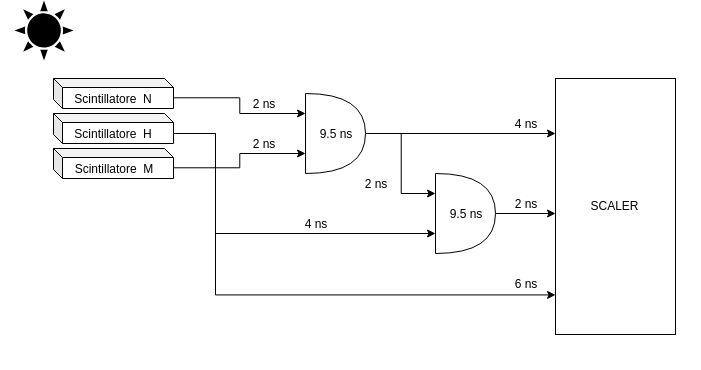
\includegraphics[width=400px]{img/conn_3.png}
\caption{Schema delle connessioni elettriche per la caratterizzazione di H.}
\label{fig:con_3}
\end{center}
\end{figure}\\
I segnali logici NIM dei vari moduli sono stati impostati in modo di avere una durata di circa 25 ns. Le misure di tensione sono state effettuate con il multimetro Meterman 35XP, con un errore di $0.5\%+1dgt$. Le misure di tempo sono state prese con il timer del modulo scaler, su un intervallo di $120.000\;s$ con un errore di 1 ms; l'errore sui conteggi è stato calcolato come la radice quadrata della misura.\\ 
\begin{figure}[h!]
\begin{center}
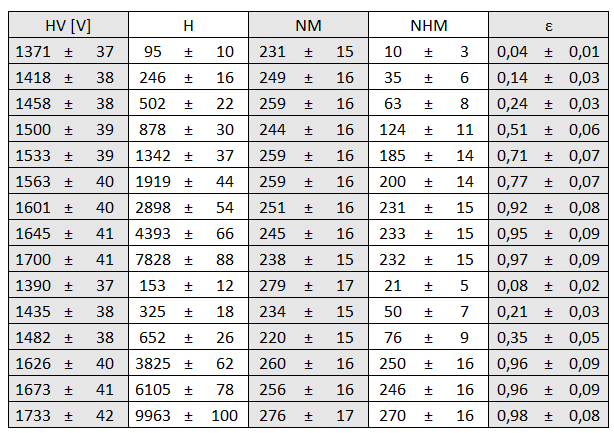
\includegraphics[width=350px]{img/table_H.png}
\caption{Misure per la curva di efficienza di H.}
\label{fig:table_H}
\end{center}
\end{figure}
\begin{figure}[!ht]
\begin{center}
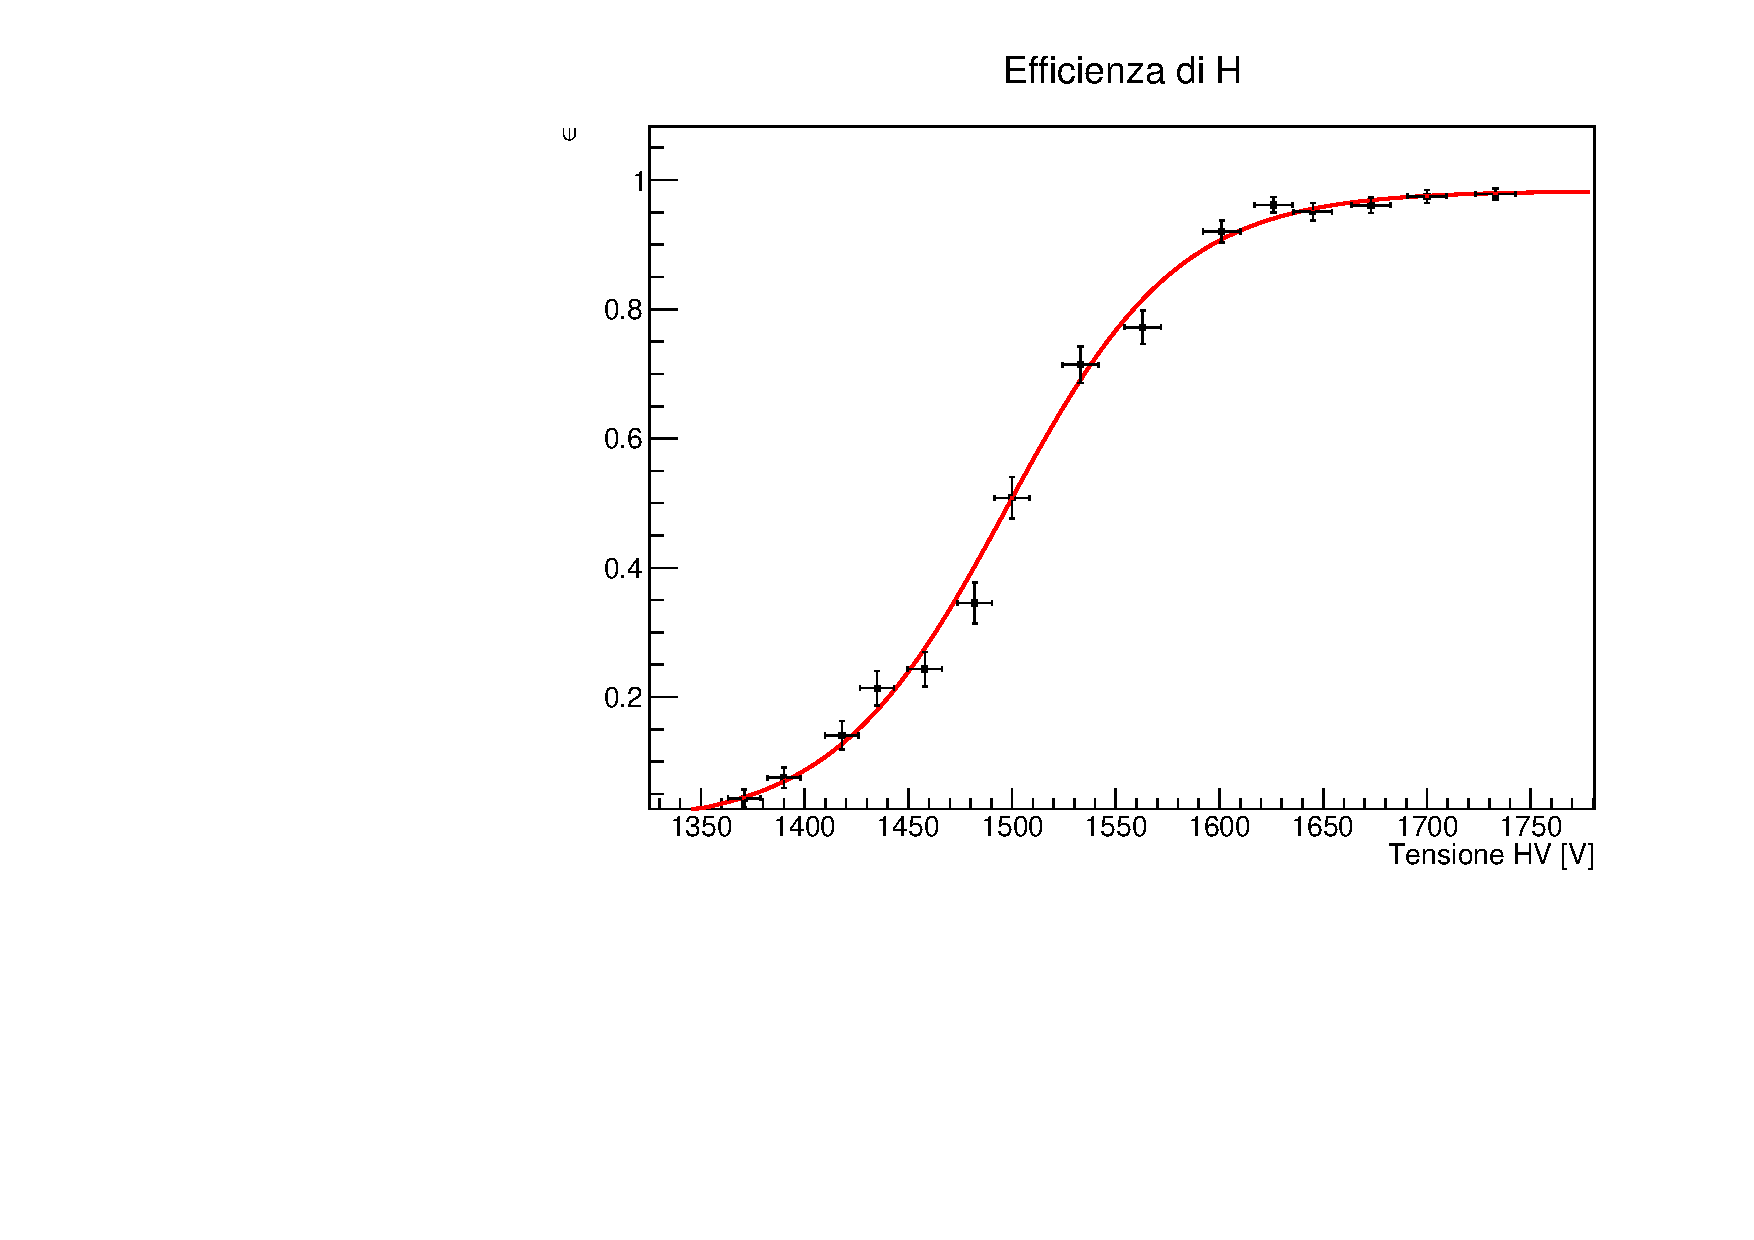
\includegraphics[width=400px]{img/chart_H.pdf}
\caption{Curva di efficienza di H.}
\label{fig:chart_H}
\end{center}
\end{figure}
\\La regressione utilizzata è la funzione:
\begin{equation}
\epsilon \left( V \right) =\frac{A}{1+e^{\frac{B-V}{C}}}
\end{equation}
dove A,B,C sono parametri liberi. Il parametro A distingue il plateau, B è l'ascissa a metà altezza e C indica la pendenza della curva.\\
\begin{table}[!h]
\begin{center}
\begin{tabular}{|c|c|c|l|}
\hline
\multicolumn{1}{|l|}{Parametro} & \multicolumn{1}{l|}{Valore} & \multicolumn{1}{l|}{Errore} & U.M. \\ \hline
A                               & 0.983                       & 0.007                       &      \\ \hline
B                               & 1497                        & 4                           & V    \\ \hline
C                               & 42                          & 2                           & V    \\ \hline
\end{tabular}
\end{center}
\caption{Risultati della regressione.}
\end{table}
\\La regressione riporta un $\chi ^2$ di 6.677 con 12 gradi di libertà ed un p-value dell'$88\%$; per cui il modello teorico descrive adeguatamente le misure sperimentali.
\begin{figure}[!h]
\begin{center}
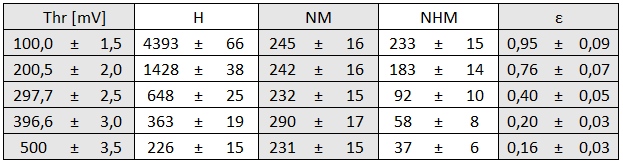
\includegraphics[width=350px]{img/thres_H.png}
\caption{Efficienza di H a diverse tensioni di lavoro.}
\label{fig:thres_H}
\end{center}
\end{figure}
\\Per questo modello di scintillatore si è scelta una tensione di lavoro di 1645 V e una soglia di 100 mV, in quanto è la configurazione dove il rapporto rumore-efficienza è minimo.\\
\\Il medesimo lavoro è stato svolto per lo scintillatore M (modello XP2232).
\begin{figure}[h!]
\begin{center}
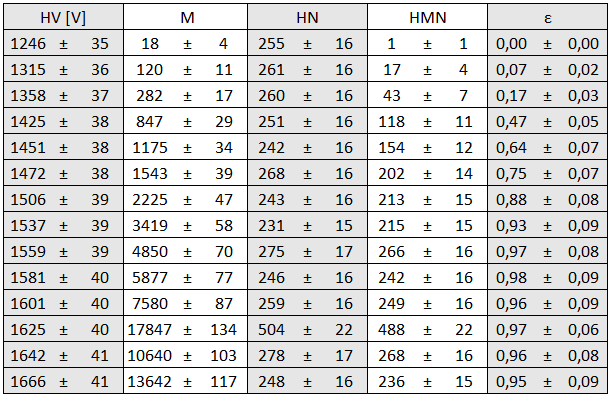
\includegraphics[width=350px]{img/table_M.png}
\caption{Misure per la curva di efficienza di M.}
\label{fig:table_M}
\end{center}
\end{figure}
\begin{figure}[!ht]
\begin{center}
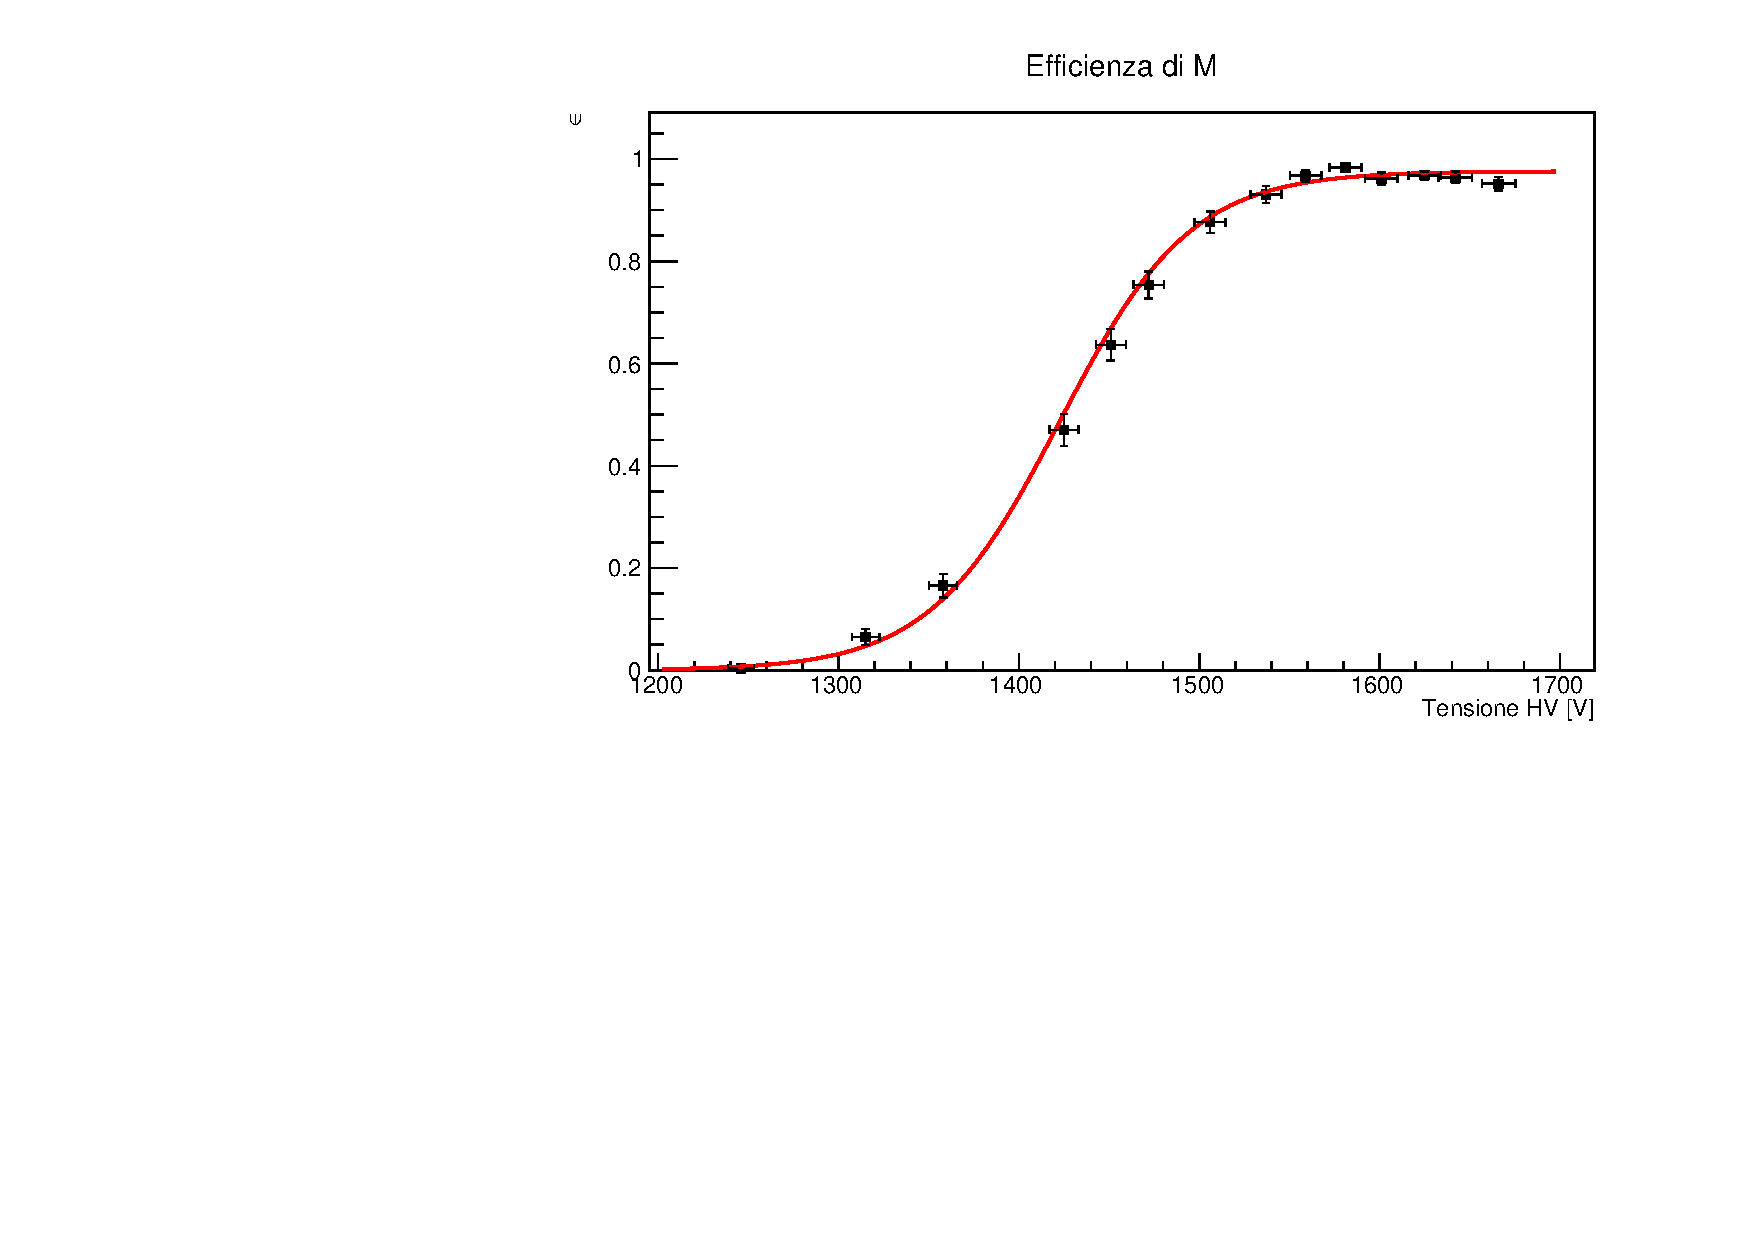
\includegraphics[width=400px]{img/chart_M.pdf}
\caption{Curva di efficienza di M.}
\label{fig:chart_M}
\end{center}
\end{figure}
\\La regressione utilizzata è la funzione (1). 
\begin{table}[!h]
\begin{center}
\begin{tabular}{|c|c|c|l|}
\hline
\multicolumn{1}{|l|}{Parametro} & \multicolumn{1}{l|}{Valore} & \multicolumn{1}{l|}{Errore} & U.M. \\ \hline
A                               & 0.976                       & 0.005                       &      \\ \hline
B                               & 1423                        & 4                           & V    \\ \hline
C                               & 36                          & 2                           & V    \\ \hline
\end{tabular}
\end{center}
\caption{Risultati della regressione.}
\end{table}
\\La regressione riporta un $\chi ^2$ di 14.23 con 11 gradi di libertà ed un p-value dell'$22\%$; per cui il modello teorico descrive adeguatamente le misure sperimentali.
\begin{figure}[!h]
\begin{center}
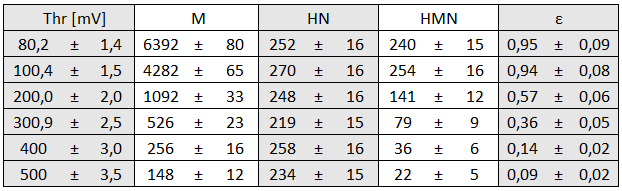
\includegraphics[width=350px]{img/thres_M.png}
\caption{Efficienza di M a diverse tensioni di lavoro.}
\label{fig:thres_H}
\end{center}
\end{figure}
\\Per questo modello di scintillatore si è scelta una tensione di lavoro di 1551 V e una soglia di 100 mV, in quanto è la configurazione dove il rapporto rumore-efficienza è minimo.\\
Per i due scintillatori I e N di tipo XP2262 (come H) si è effettuata una singola misura alla tensione di lavoro di 1645 V e soglia 100 mV.
 \begin{figure}[!h]
\begin{center}
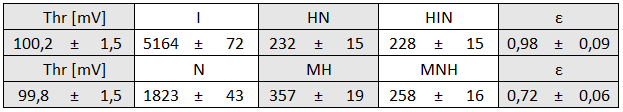
\includegraphics[width=350px]{img/thres_IN.png}
\caption{Efficienza di I e N.}
\label{fig:thres_IN}
\end{center}
\end{figure}
\\Come si può notare, lo scintillatore N non risulta essere all'efficienza massima, per cui si è scelto di effettuare una caratterizzazione completa per trovare il punto di lavoro migliore.
\begin{figure}[h!]
\begin{center}
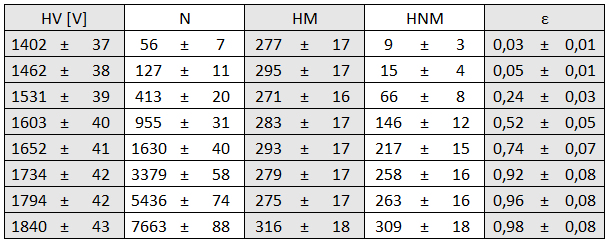
\includegraphics[width=350px]{img/table_N.png}
\caption{Misure per la curva di efficienza di N.}
\label{fig:table_N}
\end{center}
\end{figure}
\begin{figure}[!ht]
\begin{center}
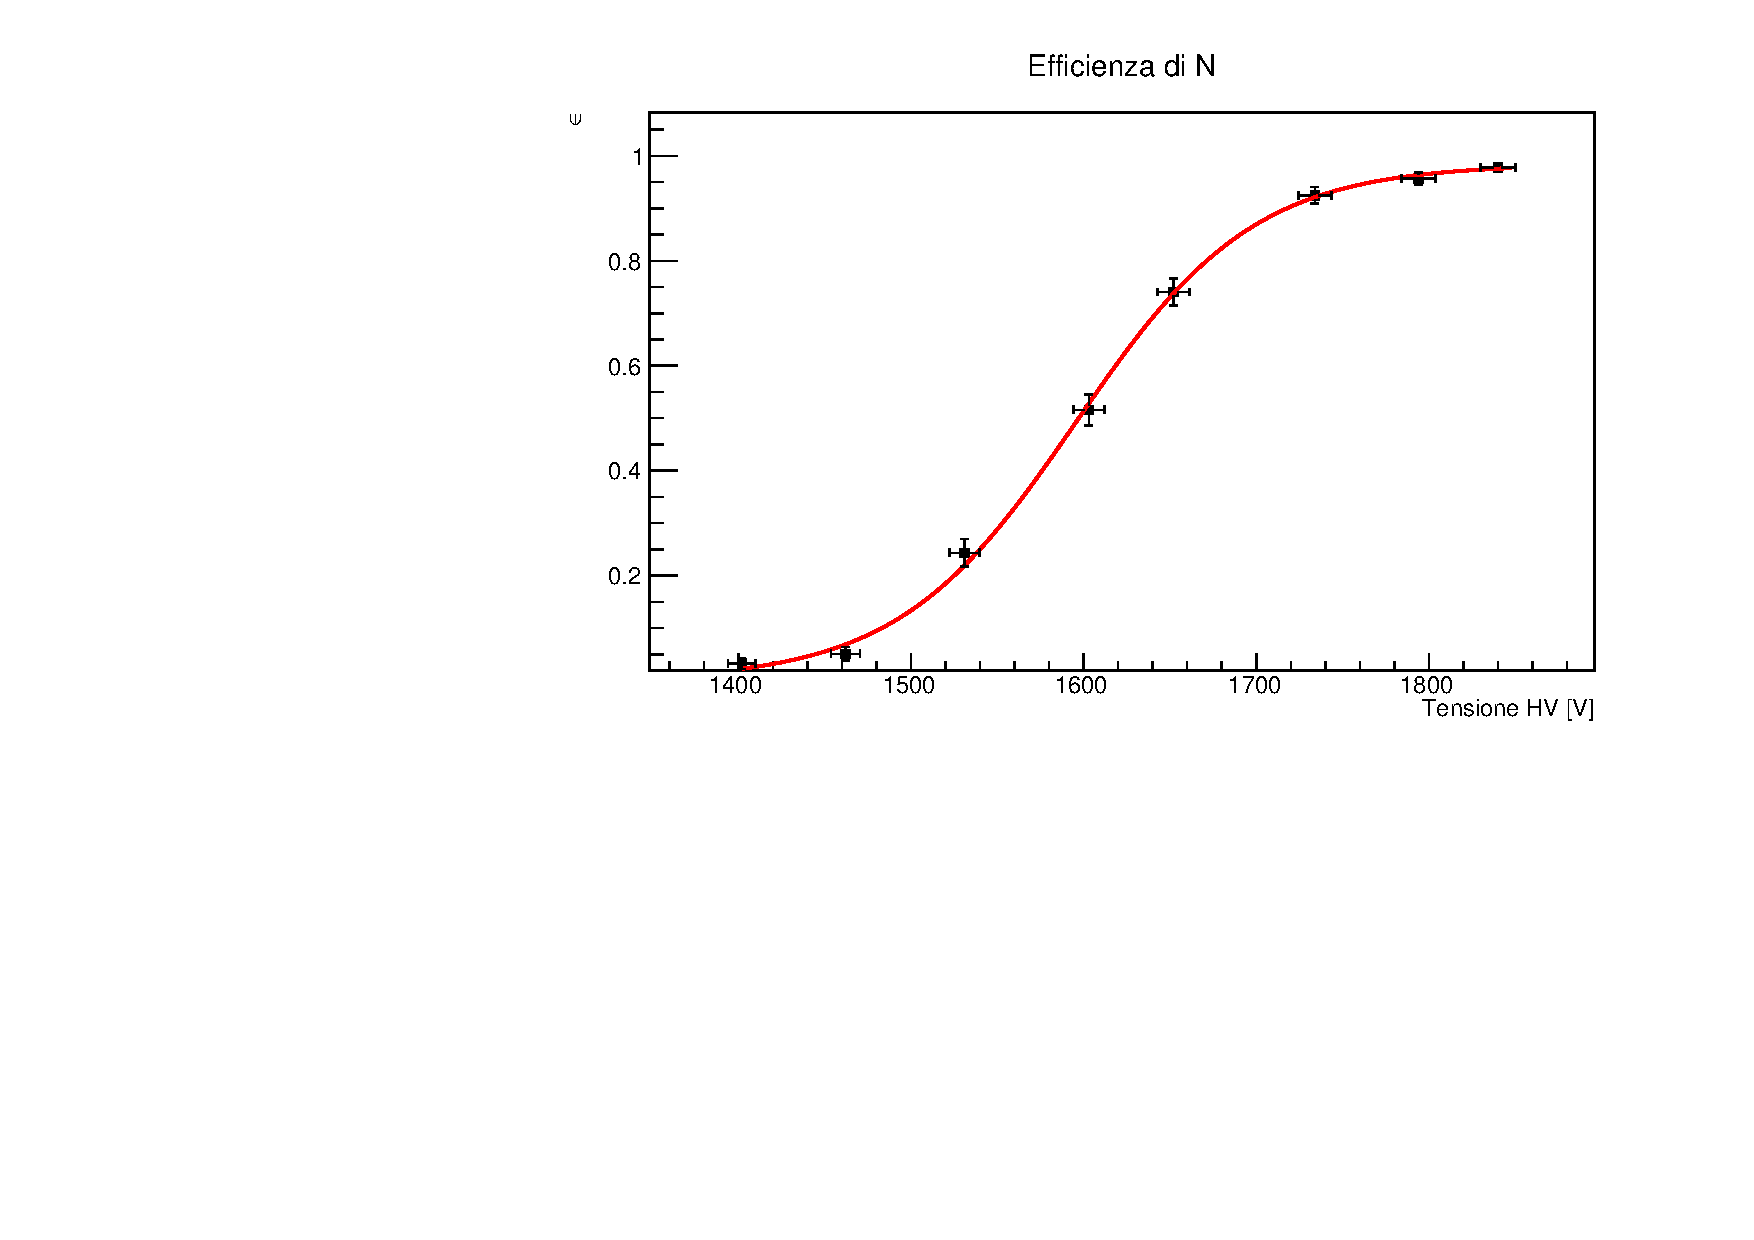
\includegraphics[width=400px]{img/chart_N.pdf}
\caption{Curva di efficienza di N.}
\label{fig:chart_N}
\end{center}
\end{figure}
\\La regressione utilizzata è la funzione (1). 
\begin{table}[!h]
\begin{center}
\begin{tabular}{|c|c|c|l|}
\hline
\multicolumn{1}{|l|}{Parametro} & \multicolumn{1}{l|}{Valore} & \multicolumn{1}{l|}{Errore} & U.M. \\ \hline
A                               & 0.984                       & 0.009                       &      \\ \hline
B                               & 1595                        & 6                           & V    \\ \hline
C                               & 52                          & 4                           & V    \\ \hline
\end{tabular}
\end{center}
\caption{Risultati della regressione.}
\end{table}
\\La regressione riporta un $\chi ^2$ di 2.85 con 5 gradi di libertà ed un p-value dell'$72\%$; per cui il modello teorico descrive adeguatamente le misure sperimentali.
\\Per questo modello di scintillatore si è scelta una tensione di lavoro di 1734 V e una soglia di 100 mV, in quanto è la configurazione dove il rapporto rumore-efficienza è minimo.\\
\subsection{Curva di coincidenza}
Per determinare quando due eventi sono coincidenti, si utilizza una porta logica AND. Per capire quali combinazioni di segnali vengono considerati coincidenti, si è effettuata una misura variando lo sfasamento fra i segnali. Per fare ciò, si sono utilizzati i moduli delay impostabili tramite selettori. Il circuito è stato costruito come segue:
\begin{figure}[h!]
\begin{center}
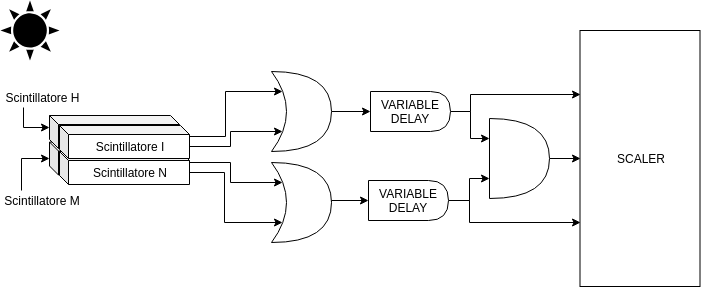
\includegraphics[width=400px]{img/conn_4.png}
\caption{Schema delle connessioni elettriche per la misura di coincidenza.}
\label{fig:con_4}
\end{center}
\end{figure}\\
In questo modo, a coppie di due rivelatori (sopra e sotto), viene operato un OR e ritardato tramite i moduli delay, i segnali in uscita vengono poi valutati tramite un AND e il tutto viene mandato allo scaler. Il delay viene fatto variare a passi di 2 ns da -34 ns a 30 ns e ogni volta il delay viene misurato tramite l'oscilloscopio (con un errore di 0.2 ns). Le misure sono state prese con intervalli di $\left(120.000\pm 0.001\right)\; ns$ tranne per la misura a 2 ns e per quelle inferiori a -27 ns di sfasamento, dove si è scelto un intervallo di $240.000\;s$ per ridurre l'errore relativo dovuto al numero di conteggi ridotto. 
\newpage
\begin{figure}[h!]
\begin{center}
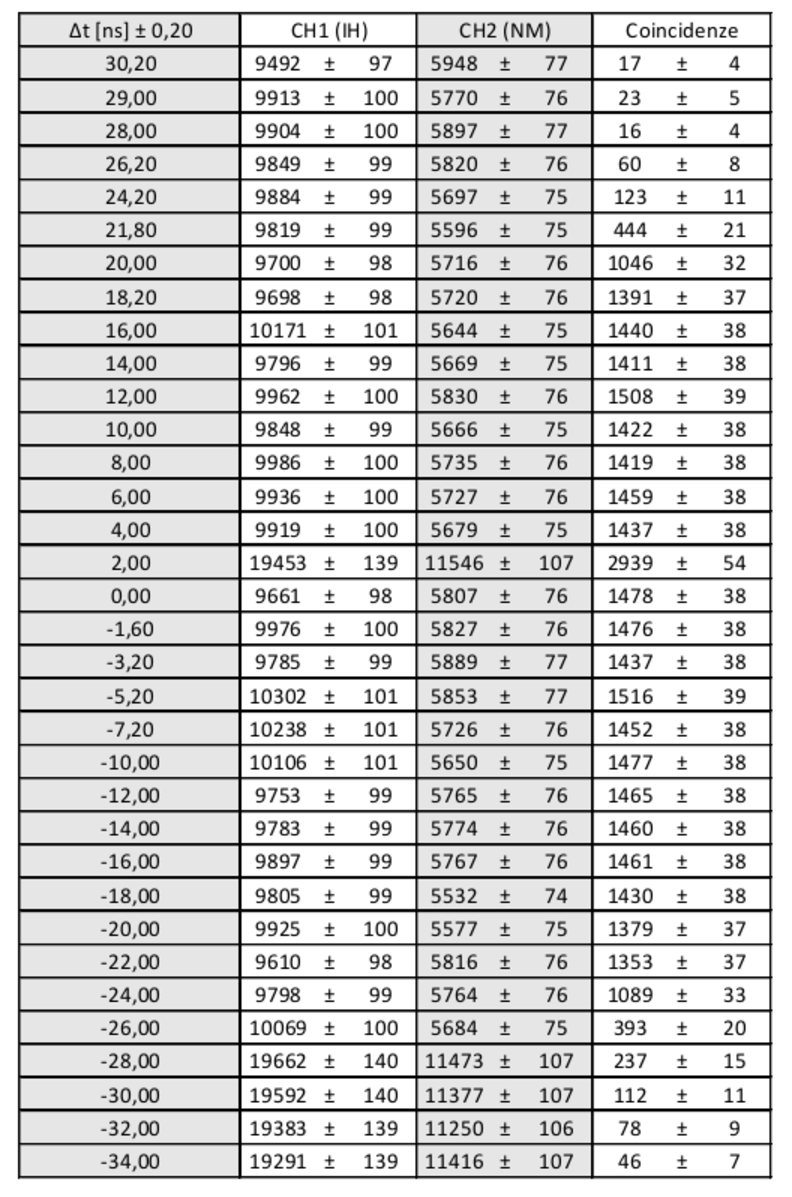
\includegraphics[width=350px]{img/table_C.pdf}
\caption{Misure per la curva di coincidenza.}
\label{fig:table_C}
\end{center}
\end{figure}
Si sono graficate le misure prese e si sono effettuate tre regressioni: una per la salita, una per il plateau e una per la discesa.
\begin{equation}
c_1\left( t \right) =\frac{A}{1+e^{\frac{B-t}{C}}},\;\;\;\;c_2  \left( t \right) = M*t+Q,\;\;\;\;c_3 \left( t \right) =\frac{D}{1+e^{\frac{t-E}{F}}},\;
\end{equation}
\newpage
\begin{figure}[h!]
\begin{center}
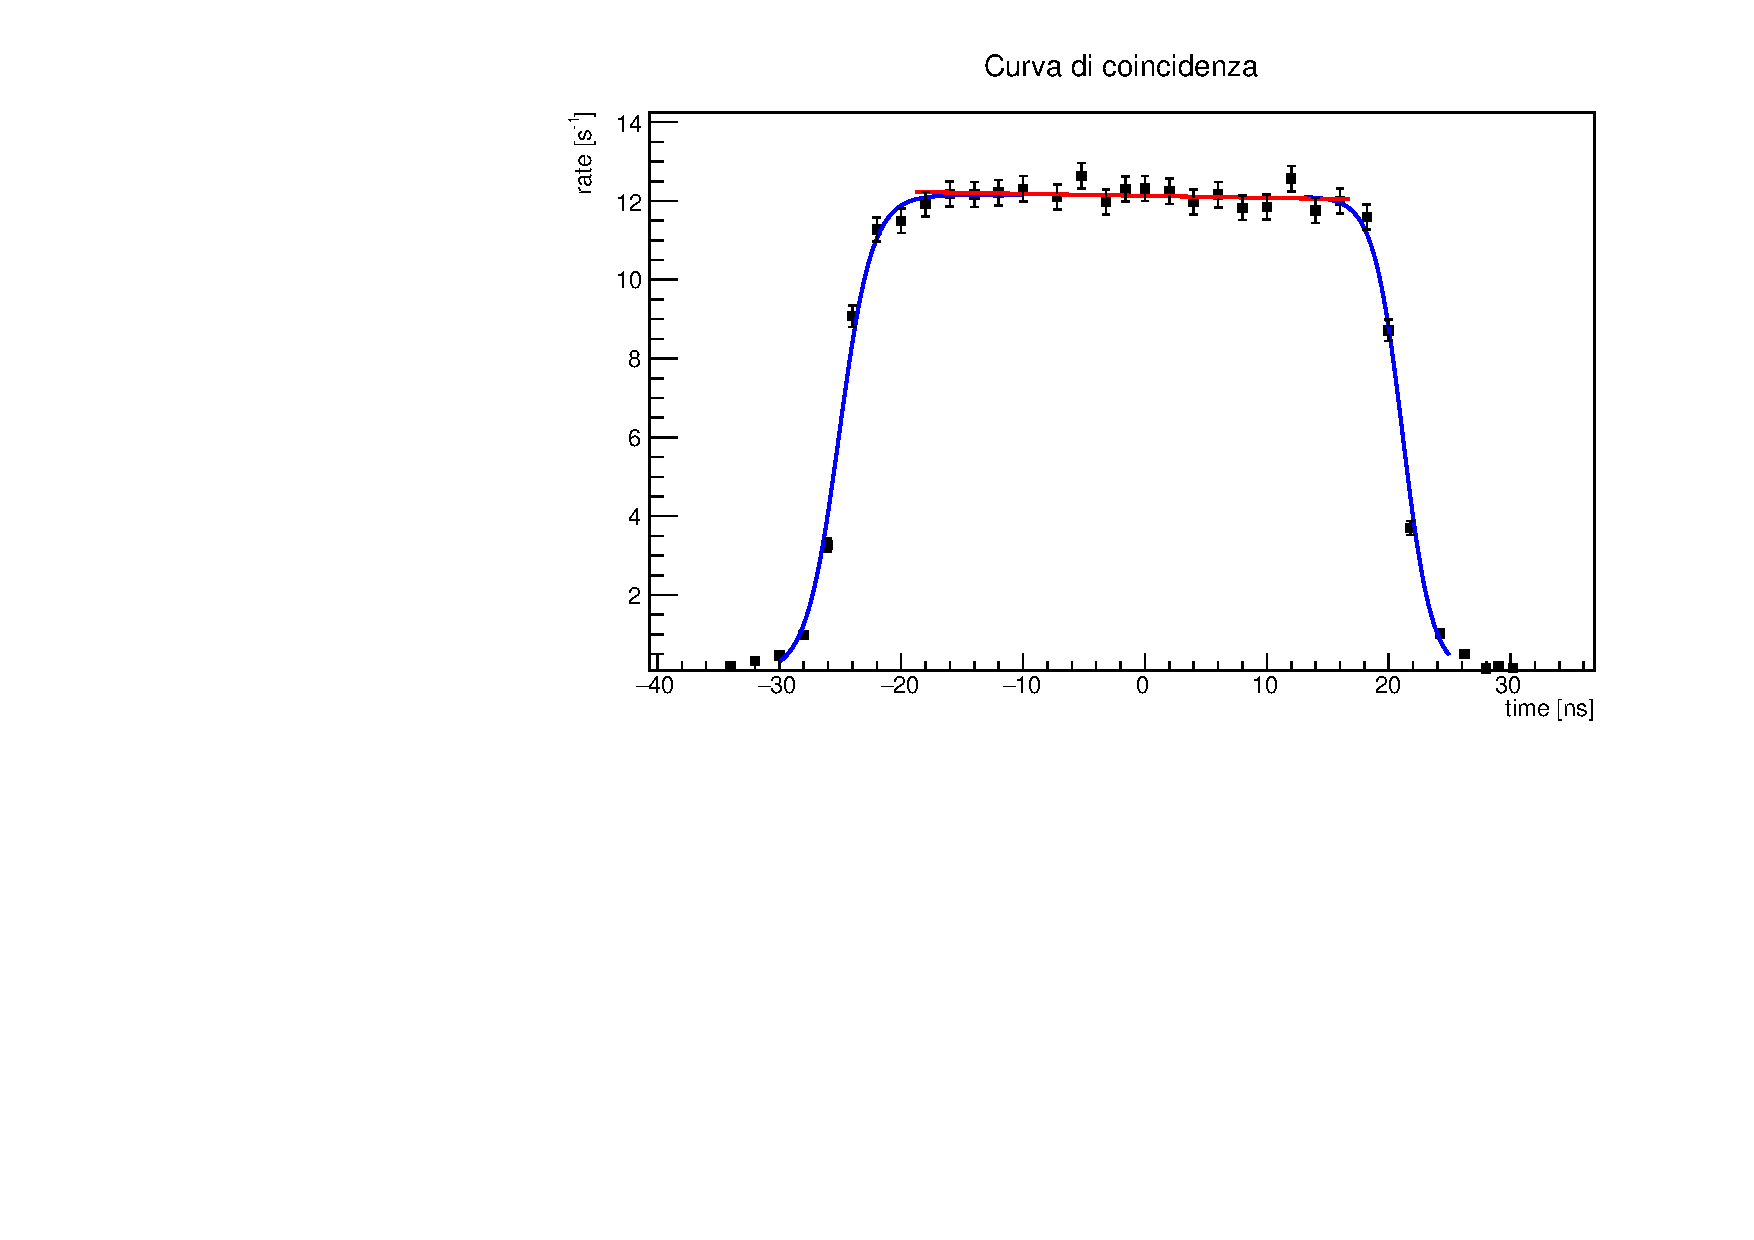
\includegraphics[width=320px]{img/chart_C.pdf}
\caption{Curva di coincidenza.}
\label{fig:coin}
\end{center}
\end{figure}
\begin{table}[!h]
\begin{center}
\begin{tabular}{|c|c|c|l|}
\hline
\multicolumn{1}{|l|}{Parametro} & \multicolumn{1}{l|}{Valore} & \multicolumn{1}{l|}{Errore} & U.M. \\ \hline
A                               & 12.1                       & 0.2                      & Hz     \\ \hline
B                               & 21.1                        & 0.2                           & $\times10^{-9}\;s$    \\ \hline
C                               & 1.3                          & 0.07                          &  $\times10^{-9}\;s$    \\ \hline
\end{tabular}
\end{center}
\caption{Risultati della regressione sulla salita [-30.20,-10.00] ns.}
\end{table}
Il modello teorico risulta compatibile con i dati con un p-value del $13\%$, $\chi ^2=5.68$ e 3 gradi di libertà.
\begin{table}[!h]
\begin{center}
\begin{tabular}{|c|c|c|l|}
\hline
\multicolumn{1}{|l|}{Parametro} & \multicolumn{1}{l|}{Valore} & \multicolumn{1}{l|}{Errore} & U.M. \\ \hline
M                               & -0.005                       & 0.007                 & $\times 10^{-9}\;s^{-2}$     \\ \hline
Q                               & 12.13                      & 0.08                           & Hz    \\ \hline
\end{tabular}
\end{center}
\caption{Risultati della regressione sul plateau  [-19.00,17.00] ns.}
\end{table}
\\Il modello teorico risulta compatibile con i dati con un p-value del $91\%$, $\chi ^2=9.14$ e 16 gradi di libertà.
\begin{table}[!h]
\begin{center}
\begin{tabular}{|c|c|c|l|}
\hline
\multicolumn{1}{|l|}{Parametro} & \multicolumn{1}{l|}{Valore} & \multicolumn{1}{l|}{Errore} & U.M. \\ \hline
D                               & 12.2                       & 0.1                       &    Hz \\ \hline
E                               & -25.1                       & 0.2                           & $\times10^{-9}\;s$    \\ \hline
F                               & 1.34                          & 0.07                           & $\times10^{-9}\;s$    \\ \hline
\end{tabular}
\end{center}
\caption{Risultati della regressione sulla discesa [13.00,25.00] ns. .}
\end{table}
\\Il modello teorico risulta compatibile con i dati con un p-value del $7\%$, $\chi ^2=14.37$ e 8 gradi di libertà.
Come si può vedere dal grafico in figura \ref{fig:coin}, la curva di coincidenza non è perfettamente centrata in zero. Lo spostamento di circa 5 ns è probabilmente dovuto a ritardi non considerati nell'elettronica di acquisizione o ad un impostazione poco precisa della durata del segnale logico (discriminatore o porte logiche).\\ Il plateau risulta compatibile con una costante ( M compatibile con 0, il test normale riporta un p-value $30\%$). Come si può notare, l'ampiezza del plateau è circa due volte la durata impostata del segnale NIM, come previsto.
\subsection{Rumore di fondo}
Mantenendo il setup del paragrafo precedente, si è impostato il delay fra i segnali a $\left(150.0\pm0.2\right)$ ns. In questo modo, si sono misurate le coincidenze completamente casuali durante l'arco notturno di $\left(20h18m\pm2m\right)$. Queste sono state comparate con il rate accidentale, calcolato come $R_{acc} =2 \mu R_{IH}R_{NM}$ dove $\mu = \left(20.0\pm0.2\right) ns$ durata del segnale NIM.\\
\begin{table}[!h]
\begin{center}
\begin{tabular}{|l|l|l|l|}
\hline
Rate IH                   & Rate NM                & Rate Accidentale & Rate Notturno   \\ \hline
\multicolumn{1}{|c|}{$\left(82\pm1\right)\; Hz$} & \multicolumn{1}{c|}{$\left(48\pm1\right)\; Hz$}& \multicolumn{1}{|c|}{$\left(159\pm5\right)\times10^{-6}\;Hz$} &\multicolumn{1}{c|}{$\left(821\pm106\right)\times10^{-6}\;Hz$}          \\ \hline
\end{tabular}
\end{center}
\caption{Comparazione Rate Accidentale e Rate Notturno.}
\end{table}
\\Come si può notare, il rate notturno risulta molto più grande di quello accidentale e quindi incompatibile (p-value = 0), sebbene sia dello stesso ordine di grandezza. Questo è possibile ricondurlo al fatto che avvengano altri fenomeni di cui non si è presa considerazione, oltre alle coincidenze accidentali.
\section{Misure con il dispositivo portatile}
\subsection{Distribuzione angolare sul tetto dell'edificio}
\begin{wrapfigure}{R}{0.35\textwidth}
\vspace{-30pt}
  \begin{center}
    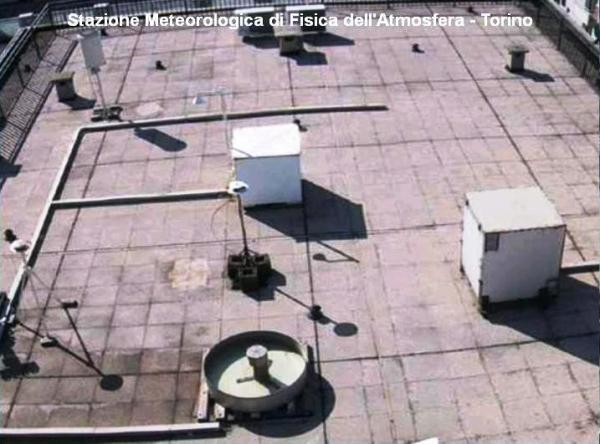
\includegraphics[width=0.35\textwidth]{img/tetto.jpg}
  \end{center}
  \caption{Tetto dell'edificio.}
\end{wrapfigure}
Per le misure con il dispositivo portatile,  si è raggiunto il tetto dell'edificio a quota 254 m (slm). Le condizioni meteo durante la giornata della presa dati erano cielo poco nuvolso (visibilità 70 km), inoltre sul tetto non erano presenti ostacoli che potessero influenzare le misurazioni.\\
Impostata la distanza fra i due scintillatori a $\left(30.0\pm0.1\right)\;cm$ e verificato sul goniometro che l'angolo fosse $\left(0\pm5\right)^{\circ}$, abbiamo iniziato a raccogliere i conteggi su un intervallo di 420 secondi circa. La misura è stata ripetuta per gli angoli $15^{\circ},30^{\circ},45^{\circ},60^{\circ}$.
\begin{figure}[h!]
\begin{center}
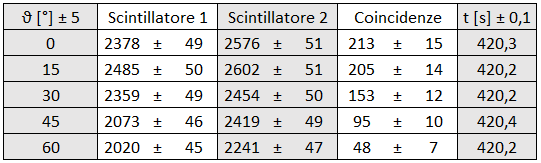
\includegraphics[width=280px]{img/CB1.PNG}
\caption{Misure della distribuzione angolare dei raggi cosmici.}
\label{fig:CBangle}
\end{center}
\end{figure}
\begin{figure}[h!]
\begin{center}
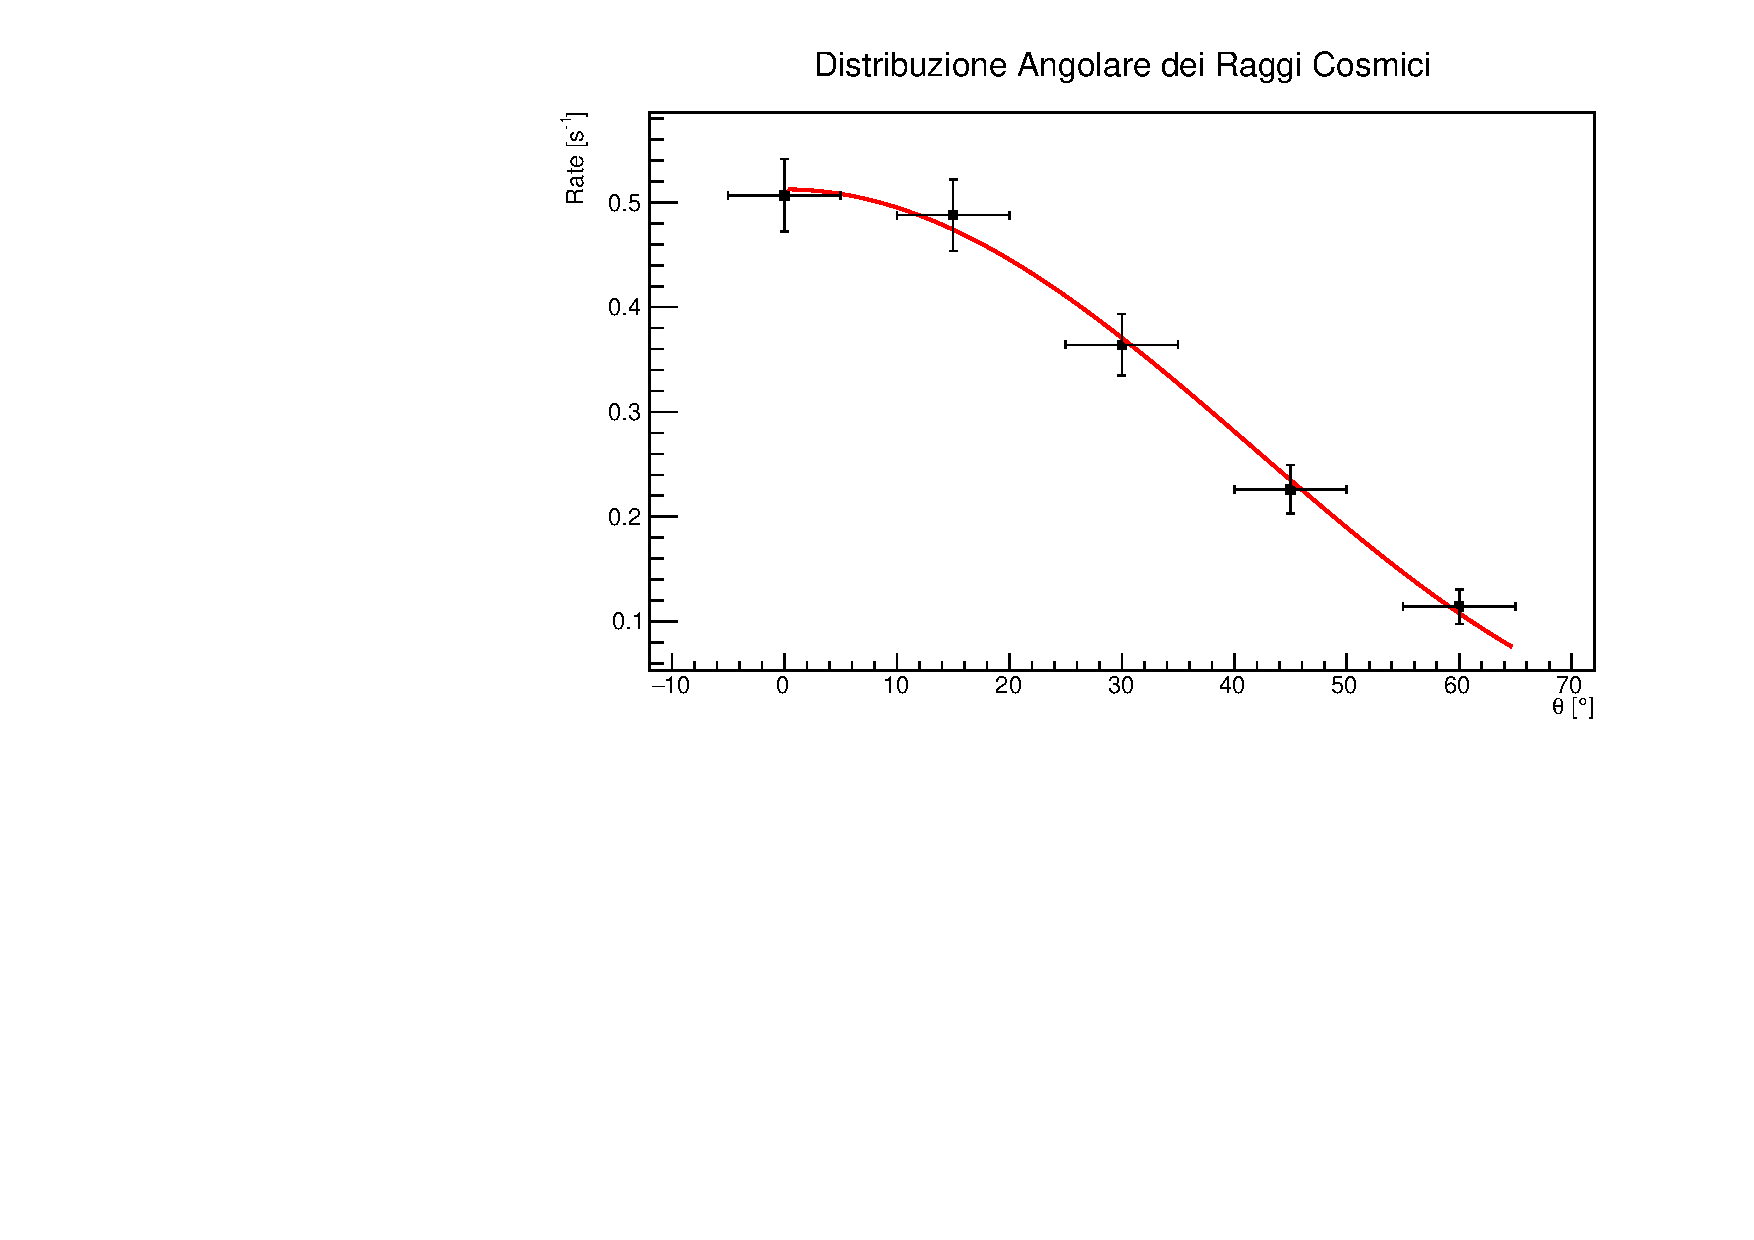
\includegraphics[width=300px]{img/CBdeg.pdf}
\caption{Distribuzione angolare dei raggi cosmici.}
\label{fig:CBdeg}
\end{center}
\end{figure}
\\La funzione utilizzata per la regressione dei dati è
\begin{equation}
R\left(\theta\right)=R_{0}\,cos\,^{n}\left(\theta\right)
\end{equation}
dove $R_0$ è il rate in posizione verticale e $n$ l'esponente del coseno.
\begin{table}[!h]
\begin{center}
\begin{tabular}{|c|c|c|l|}
\hline
\multicolumn{1}{|l|}{Parametro} & \multicolumn{1}{l|}{Valore} & \multicolumn{1}{l|}{Errore} & U.M. \\ \hline
$R_0$                               & 0.51                       & 0.03                       &    Hz \\ \hline
$n$                               & 2.3                       & 0.4                           &    \\ \hline
\end{tabular}
\end{center}
\caption{Risultati della regressione.}
\end{table}
\\Il fit ha dato risutato positivo, con un $\chi ^2 = 0.21$, p-value = 0.98 e 3 gradi di libertà. L'esponente del coseno risulta compatibile con il valore atteso di 2 (p-value = 0.28). 
\subsection{Coefficiente di assorbimento dell'edificio}
Per determinare il coefficiente di assorbimento dell'edificio, abbiamo raccolto i conteggi a diversi piani dell'edificio nuovo di fisica fissando la distanza tra gli scintillatori a $\left(12.5\pm0.1\right)\;cm$ e il tempo a circa 300 secondi; eccetto per i conteggi sul tetto per i quali abbiamo mantenuto i dati già acquisiti.
\begin{figure}[h!]
\begin{center}
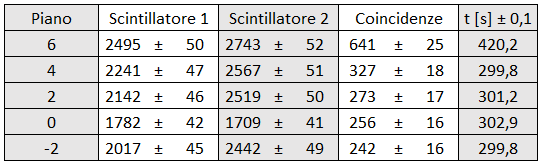
\includegraphics[width=280px]{img/CB4.PNG}
\caption{Conteggi e coincidenze raccolte ai vari piani.}
\label{fig:CBa}
\end{center}
\end{figure}
\begin{figure}[h!]
\begin{center}
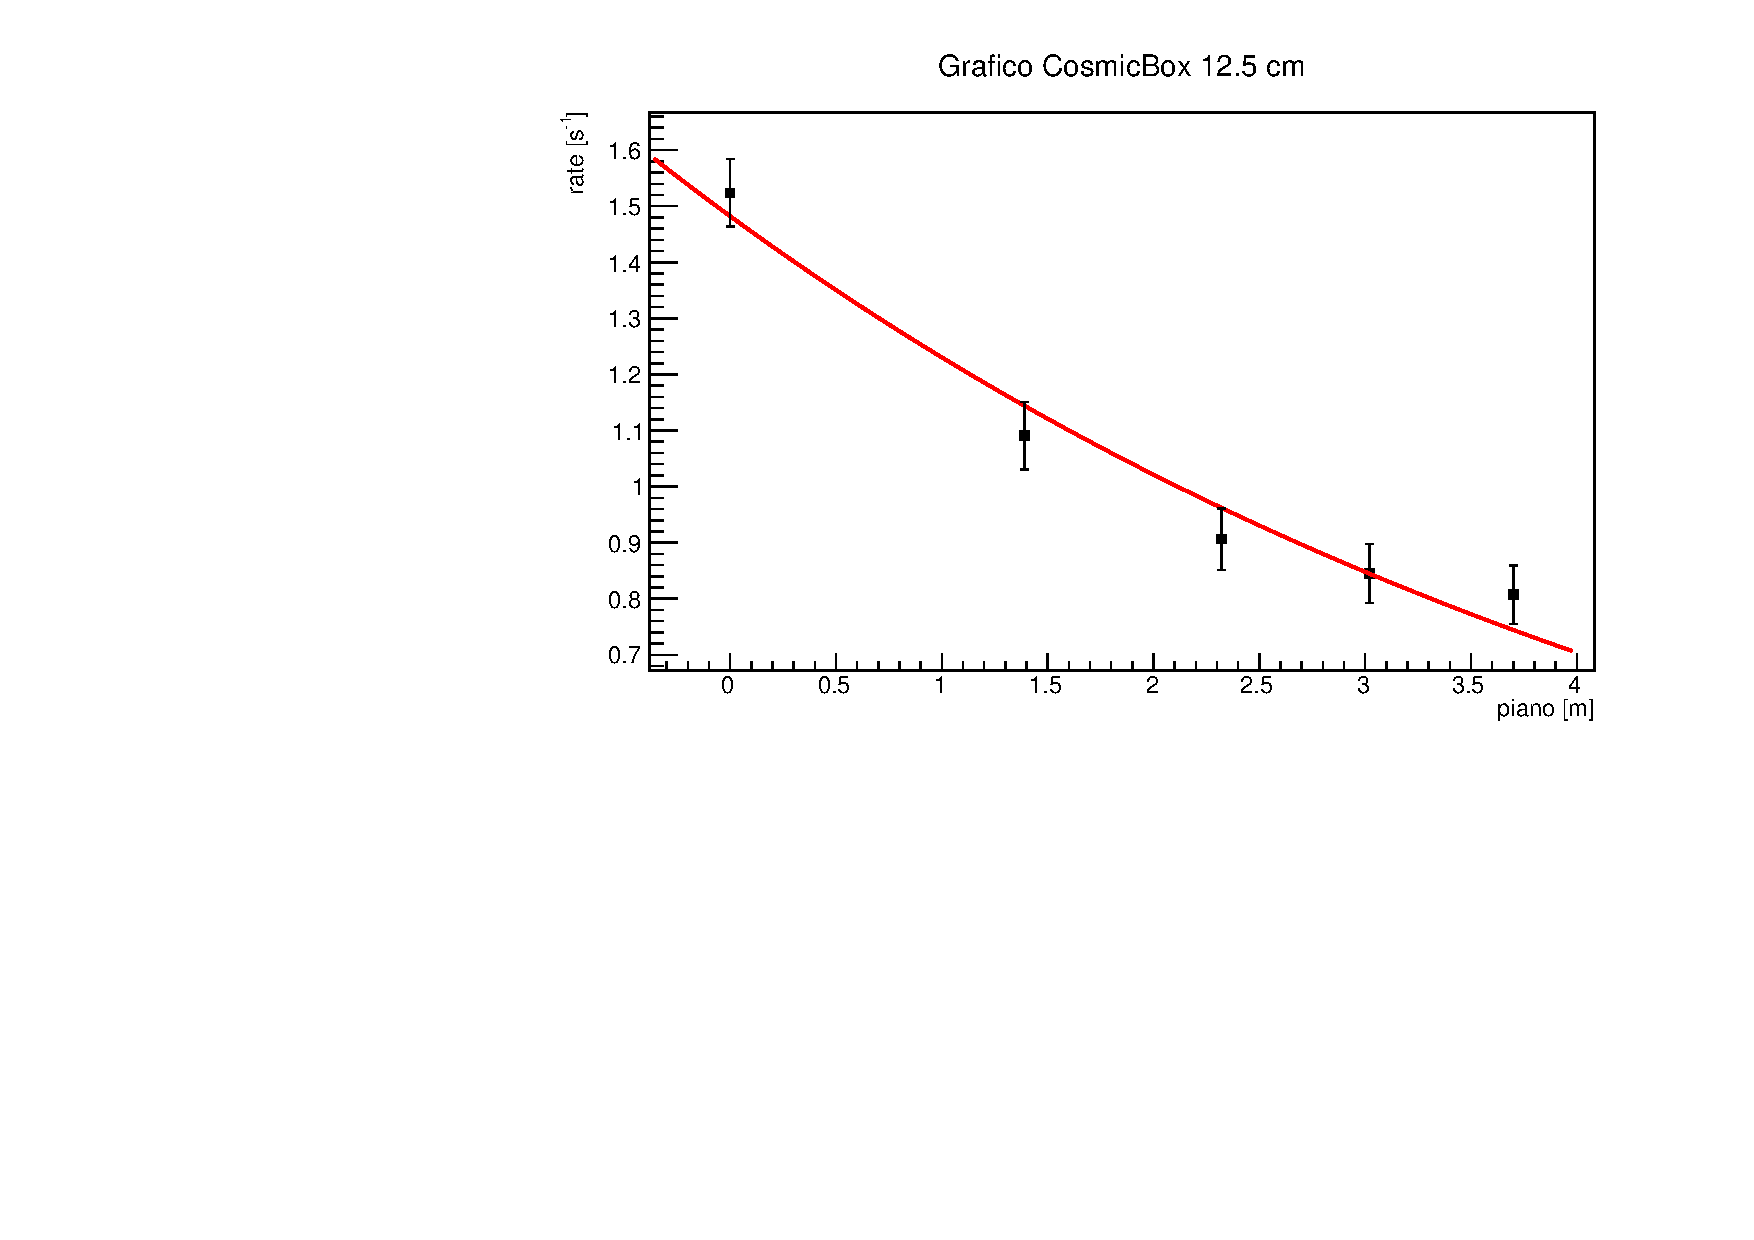
\includegraphics[width=300px]{img/CBexp.pdf}
\caption{Grafico di assorbimento dei raggi cosmici.}
\label{fig:CBexp}
\end{center}
\end{figure}
\\\\ L'altezza dei vari piani è stata determinata tramite la planimetria trasversale dell'edificio, assumendo solamente gli spessori delle solette. La funzione utilizzata per il fit è
\begin{equation}
R\left(x\right)=R_{0}\,e\,^{-\alpha x}
\end{equation}
dove $R_0$ è il rate ideale e $\alpha$ è il coefficiente di attenuazione.
\begin{table}[!h]
\begin{center}
\begin{tabular}{|c|c|c|l|}
\hline
\multicolumn{1}{|l|}{Parametro} & \multicolumn{1}{l|}{Valore} & \multicolumn{1}{l|}{Errore} & U.M. \\ \hline
$R_0$                               & 1.48                       & 0.06                       &    Hz  \\ \hline
$\alpha$                               & 0.19                       & 0.02                          & $m^{-1}$   \\ \hline
\end{tabular}
\end{center}
\caption{Risultati della regressione.}
\end{table}
\\Quindi si è calcolato il fattore di attenuazione $\eta$ come $R_{-2}/R_{6}$ e come $e^{-\alpha x_{TOT}}$.
\begin{table}[!h]
\begin{center}
\begin{tabular}{|c|c|c|l|}
\hline
\multicolumn{1}{|l|}{$\eta\;\left(R_{-2}/R_{6}\right)$} & \multicolumn{1}{l|}{$\eta\;\left(e^{-\alpha x_{TOT}}\right)$}  & p-value \\ \hline
$$ $\left(0.53\pm0.04\right)$                               & $\left(0.495\pm0.002\right)$                      &38\%   \\ \hline
\end{tabular}
\end{center}
\caption{Confronto dei fattori di attenuazione}
\end{table}
\\Il calcolo del fattore di attenuazione dà risultati compatibili con entrambi i metodi, benché il risultato ottenuto dalla regressione sia più accurato.
\subsection{Accettanza}
Per valutare l'accettanza della postazione fissa, si sono utilizzati i dati presi ai vari piani con l'apparato portatile per determinare se il calcolo fosse compatibile con la simulazione statistica. Nonostante la simulazione assuma che i rivelatori abbiano spessore trascurabile, i risultati risultano compatibili, per cui è appropriato utilizzare il risultato statistico per determinare l'accettanza della postazione fissa. La simulazione Monte Carlo è stata svolta con 50'000'000 interazioni.
\begin{figure}[h!]
\begin{center}
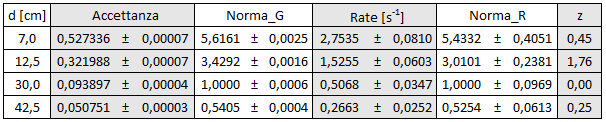
\includegraphics[width=400px]{img/table_ACC.png}
\caption{Comparazione dell'accettanza teorica e il calcolo sperimentale.}
\label{fig:ACC}
\end{center}
\end{figure}
\\L'accettanza per la postazione fissa teorica è $G=\left(0.75410\pm0.00002\right)$.
\subsection*{Risultati finali}
I risultati dei calcoli e delle misure fatte in precedenza sono stati utilizzati per determinare il valore atteso di rate e confrontarlo con quello misurato sperimentalmente. Assunto un flusso di raggi cosmici sulla superficie terrestre al livello del mare $\Phi_{teor}=180\;Hz\cdot m^{-2}$, si è calcolato il rate considerando la superficie della postazione fissa ($S=0.2 m^2$) e assumendo $\eta=\left(0.495\pm0.002\right)$ dal fit esponenziale. Per il calcolo del rate sperimentale, si è trascurato il rate di fondo, in quanto di diversi ordini di grandezza più piccolo del rate misurato; per il rate misurato si è utilizzato il valore estratto dal fit lineare del plateau ($12.13\pm 0.08$). L'efficienza della postazione è stata determinata come 
\begin{equation}
\epsilon = \left(\epsilon_I + \epsilon_H\right)\cdot\left(\epsilon_N+\epsilon_M\right)/4 = \left(0.9\pm0.2\right)
\end{equation}
per $G$ il valore statistico determinato con la simulazione $G=\left(0.75410\pm0.00002\right)$.
\begin{equation}
R_{att}= \eta\,\cdot\,R_{slm}\;,\;\;\;\;\;\;R_{sper}=\frac{R_{mis}-R_{acc}}{\epsilon \,\cdot\,G}
\end{equation}
\begin{table}[!h]
\begin{center}
\begin{tabular}{|c|c|c|c|}
\hline
\multicolumn{1}{|l|}{$R_{att}\;\left[Hz\right]$} & \multicolumn{1}{l|}{$R_{sper}\;\left[Hz\right]$} & \multicolumn{1}{l|}{Z} & p-value \\ \hline
$\left(18\pm2\right)$ & $\left(17.9\pm0.2\right)$& 0.06& 96\%\\ \hline
\end{tabular}
\end{center}
\end{table}
\\Il rate atteso di raggi cosmici risulta compatibile con quello calcolato dalle misure fatte nei paragrafi precedenti, con un p-value del 96\%.
\newpage
\section{Testbench SiPM} 
\subsection{Misura del rumore di fondo}
Utilizzando il kit SiPM della CAEN è stato osservato tramite oscilloscopio il segnale analogico senza sorgente luminosa per individuare la soglia corrispondente al primo, secondo e terzo fotoelettrone. Per tutta l'esperienza la temperatura del SiPM è rimasta stabile a $25^{\circ}$C.
\begin{figure}[h!]
\begin{center}
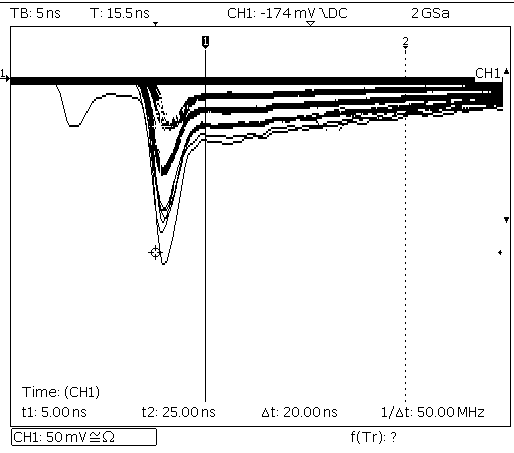
\includegraphics[width=230px]{img/SIPM01.PNG}
\caption{Segnale in uscita dal SiPM, si possono vedere chiaramente i livelli relativi ai fotoelettroni emessi.}
\label{fig:Sipm}
\end{center}
\end{figure}
\\Si è verificato che, al variare del Gain, il grafico a scalini riportasse frequenze compatibili per i primi tre livelli energetici. Si sono assunti come errori la cifra meno significativa; per le misure di frequenza, sopra i 10 kHz si è assunto un errore dell'1\%, sopra 1 kHz 5\%, 10\% altrimenti.
\begin{figure}[h!]
\begin{center}
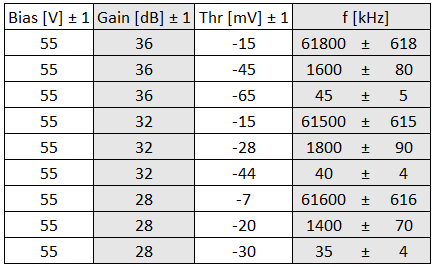
\includegraphics[width=280px]{img/tabnoise.png}
\caption{Misure di frequenza per i primi tre livelli di energia.}
\label{fig:Sipm}
\end{center}
\end{figure}
\\
L'Optical Cross Talk ai diversi Gain è costante a circa 3\%,  come da manuale.
\subsection{Misura della distribuzione energetica di una sorgente LED}
Rimosso il tappo e connessa la fibra ottica, si sono effettuate due misurazioni dello spettro di fotoelettroni emessi impostando la manopola dell'emettitore LED a 2.5 e 3.3.\\La lunghezza d'onda dei fotoni emessi è di 450 nm.
Le impostazioni utilizzate per il digitizer sono
\begin{table}[!h]
\begin{center}
\begin{tabular}{|c|c|c|l|}
\hline
\multicolumn{1}{|l|}{Parametro} & \multicolumn{1}{l|}{Valore} & \multicolumn{1}{l|}{Errore} & U.M. \\ \hline
Bias                               &55                       & 1                       & V\\ \hline
Gain                               & 32                       & 1                          & dB   \\ \hline
Gate                               & 304                       & 5                       & ns \\ \hline
Pre-Gate                               & 104                     & 5                        & ns   \\ \hline
Hold-off                               & 504                     & 5                         & ns \\ \hline
Threshold                               & 8                      & 1                          & mV   \\ \hline
No flat                               & 512                       & 5                         & ns   \\ \hline
Rise Time                               & 8                       & 1                          & ns  \\ \hline
\end{tabular}
\end{center}
\caption{Impostazioni del Digitizer.}
\end{table}
\\
In laboratorio è stata svolta una prima parte di analisi approssimativa, per stabilire i valori dei parametri per i fit.
\begin{figure}[h!]
\begin{center}
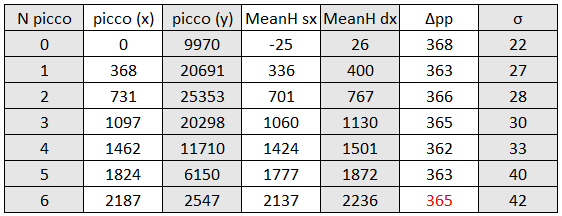
\includegraphics[width=270px]{img/tab25.png}
\caption{Misure di spettro per il LED a 2.5, in rosso $<\!\!\Delta_{pp}\!\!>$.}
\label{fig:Sipm25}
\end{center}
\end{figure}
\begin{figure}[h!]
\begin{center}
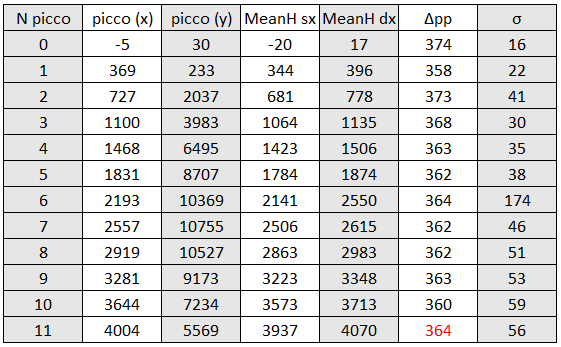
\includegraphics[width=270px]{img/tab33.png}
\caption{Misure di spettro per il LED a 3.3, in rosso $<\!\!\Delta_{pp}\!\!>$.}
\label{fig:Sipm33}
\end{center}
\end{figure}
\\Utilizzando il fit multipicco i risultati sono stati deludenti: a 2.5, il gain è troppo basso e le curve risultano tagliate verso lo zero, delineando solamente le punte del picco, mentre a 3.3 il setup si ritrova in una situazione limite, in quanto il segnale presenta un forte rumore di fondo. Si è provato successivamente il fit di una curva gaussiana per singoli picchi, ma anche questi hanno riportato risultati pessimi con p-value di zero.
\begin{figure}[!h]
\centering
    \subfloat[]{{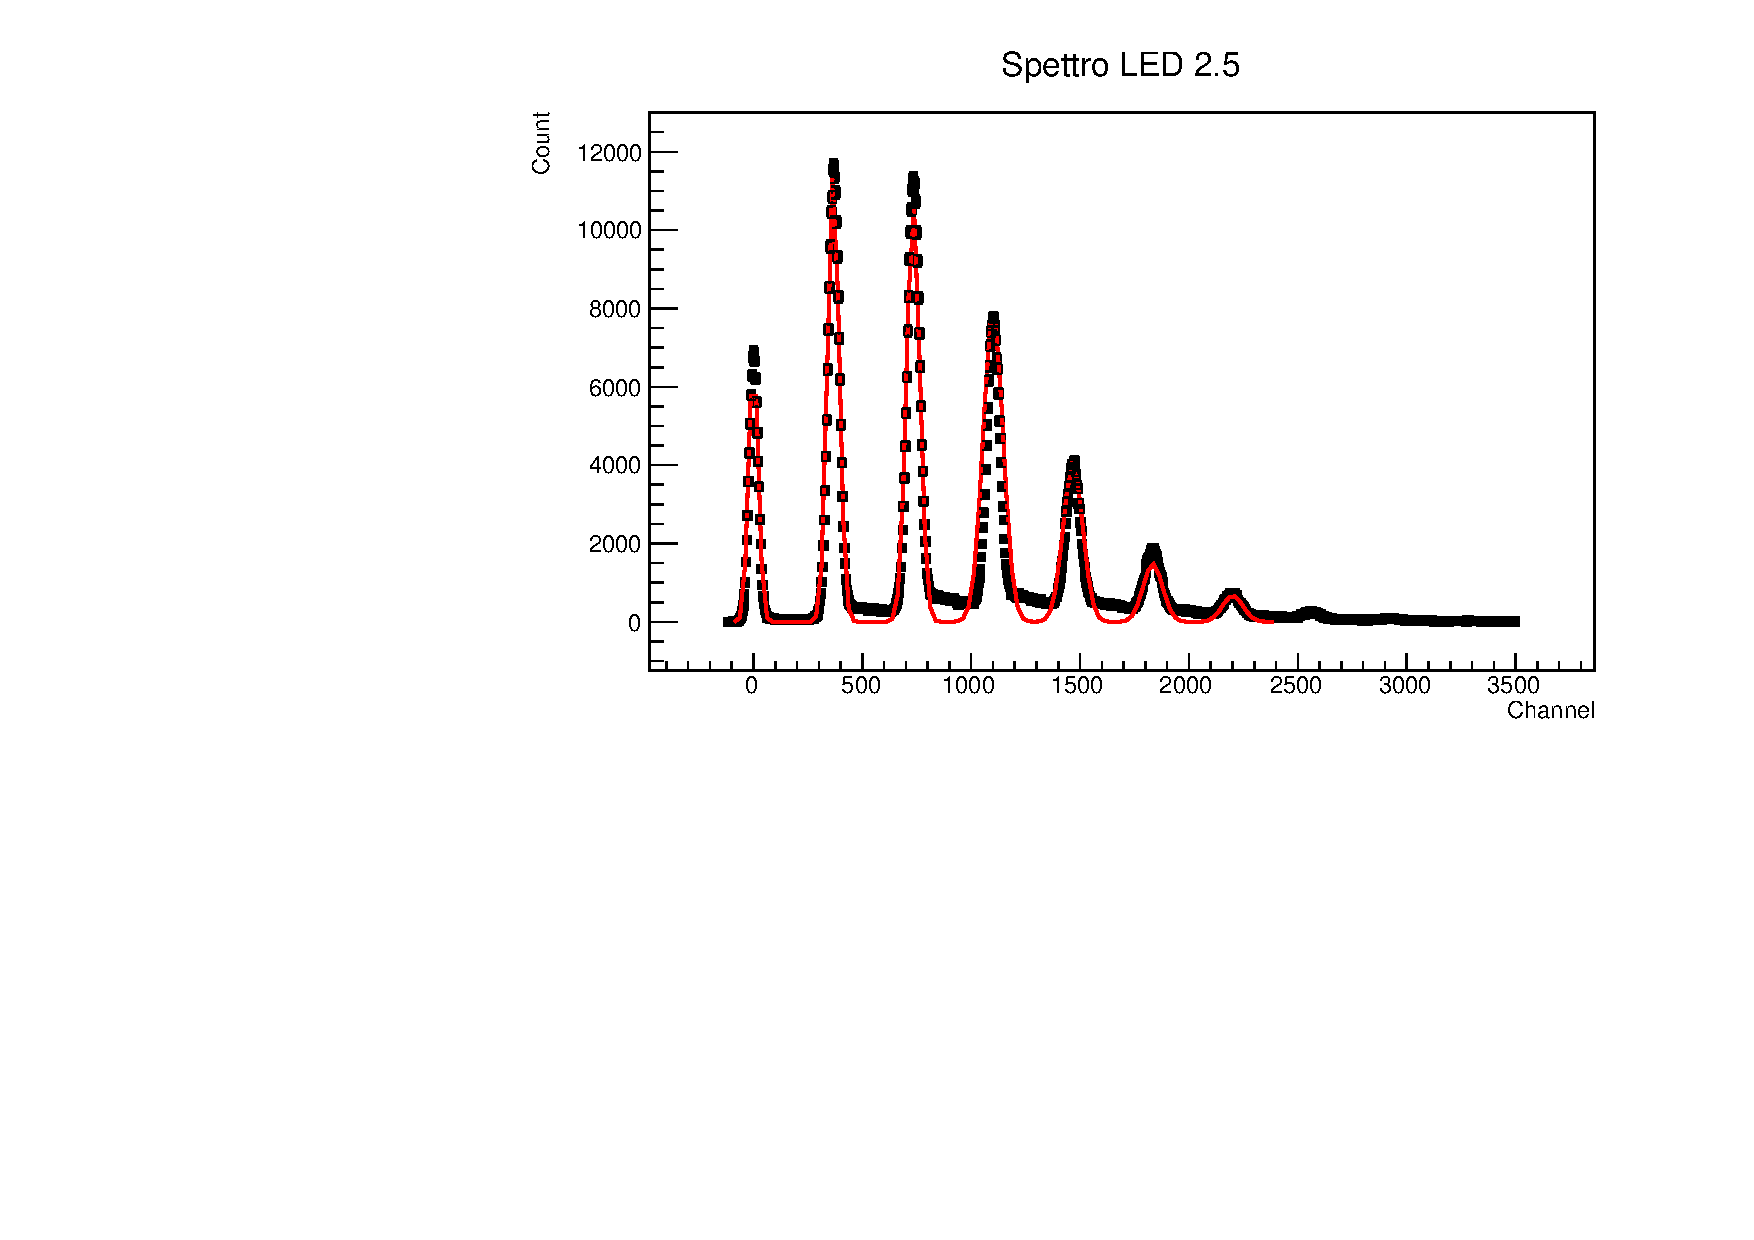
\includegraphics[width=7.5cm]{img/multi25.pdf} }}%
    \subfloat[]{{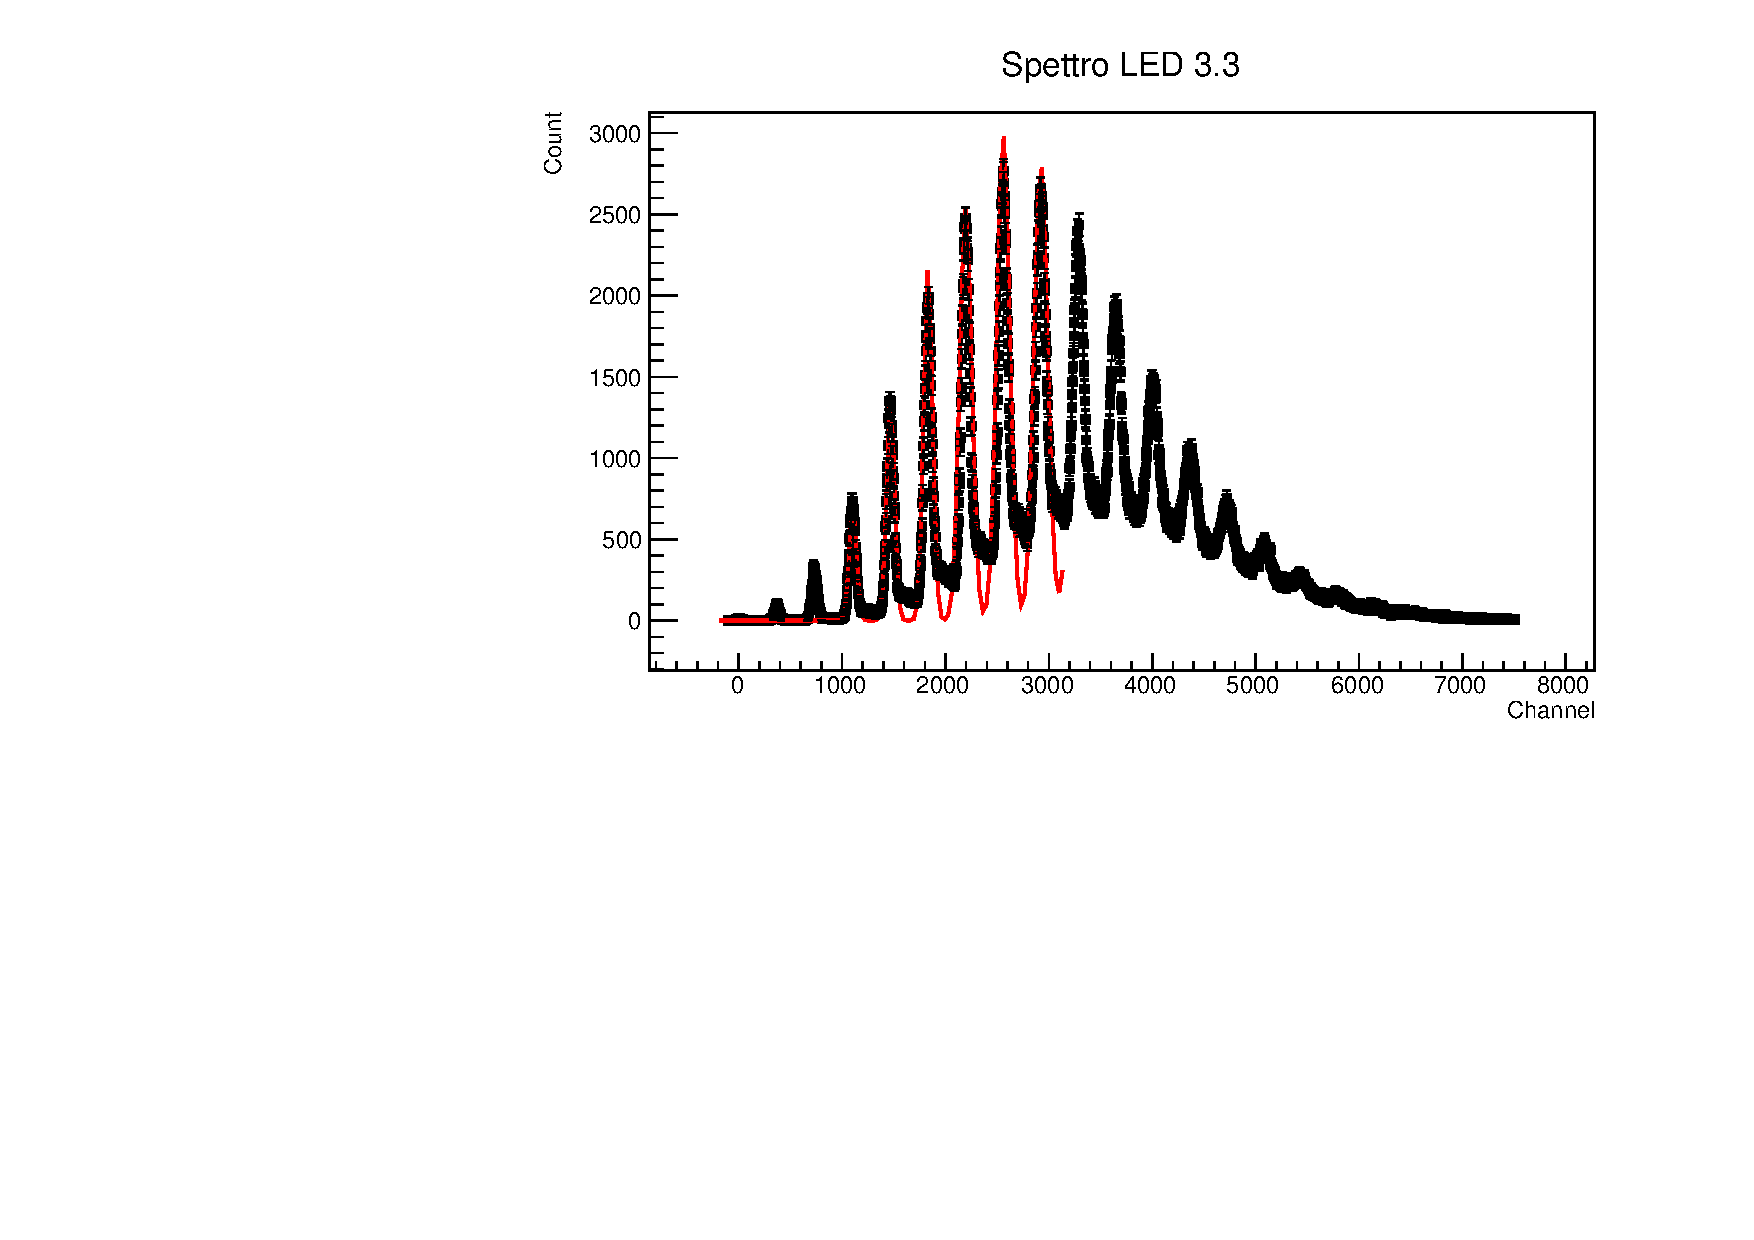
\includegraphics[width=7.5cm]{img/multi33.pdf} }}%
\caption{Fit multipicco falliti sugli spettri emessi.}
\end{figure}
\\ Si è quindi optato per cercare manualmente le coordinate dei centri e i FWHM di ogni picco per poi proced i centriere con il fit di una distribuzione di Poisson sull'integrale dei picchi, calcolato come $N_i\cdot\sigma_i \sqrt{2\pi}$. 
\begin{figure}[h!]
\begin{center}
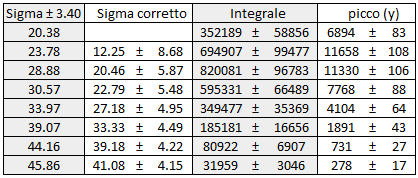
\includegraphics[width=260px]{img/tabp25.PNG}
\caption{Determinazione manuale dei valori delle gaussiane sui picchi per lo spettro a 2.5.}
\label{fig:tabpicchi25}
\end{center}
\end{figure}
\begin{figure}[h!]
\begin{center}
\vspace{-41pt}
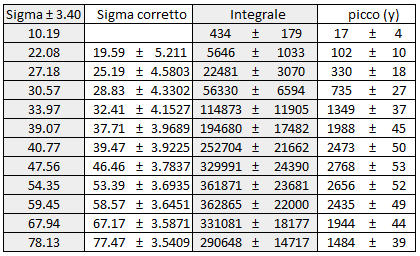
\includegraphics[width=260px]{img/tabp33.PNG}
\caption{Determinazione manuale dei valori delle gaussiane sui picchi per lo spettro a 3.3.}
\label{fig:tabpicchi25}
\end{center}
\end{figure}
\newpage
\begin{figure}[!h]
\centering
    \subfloat[]{{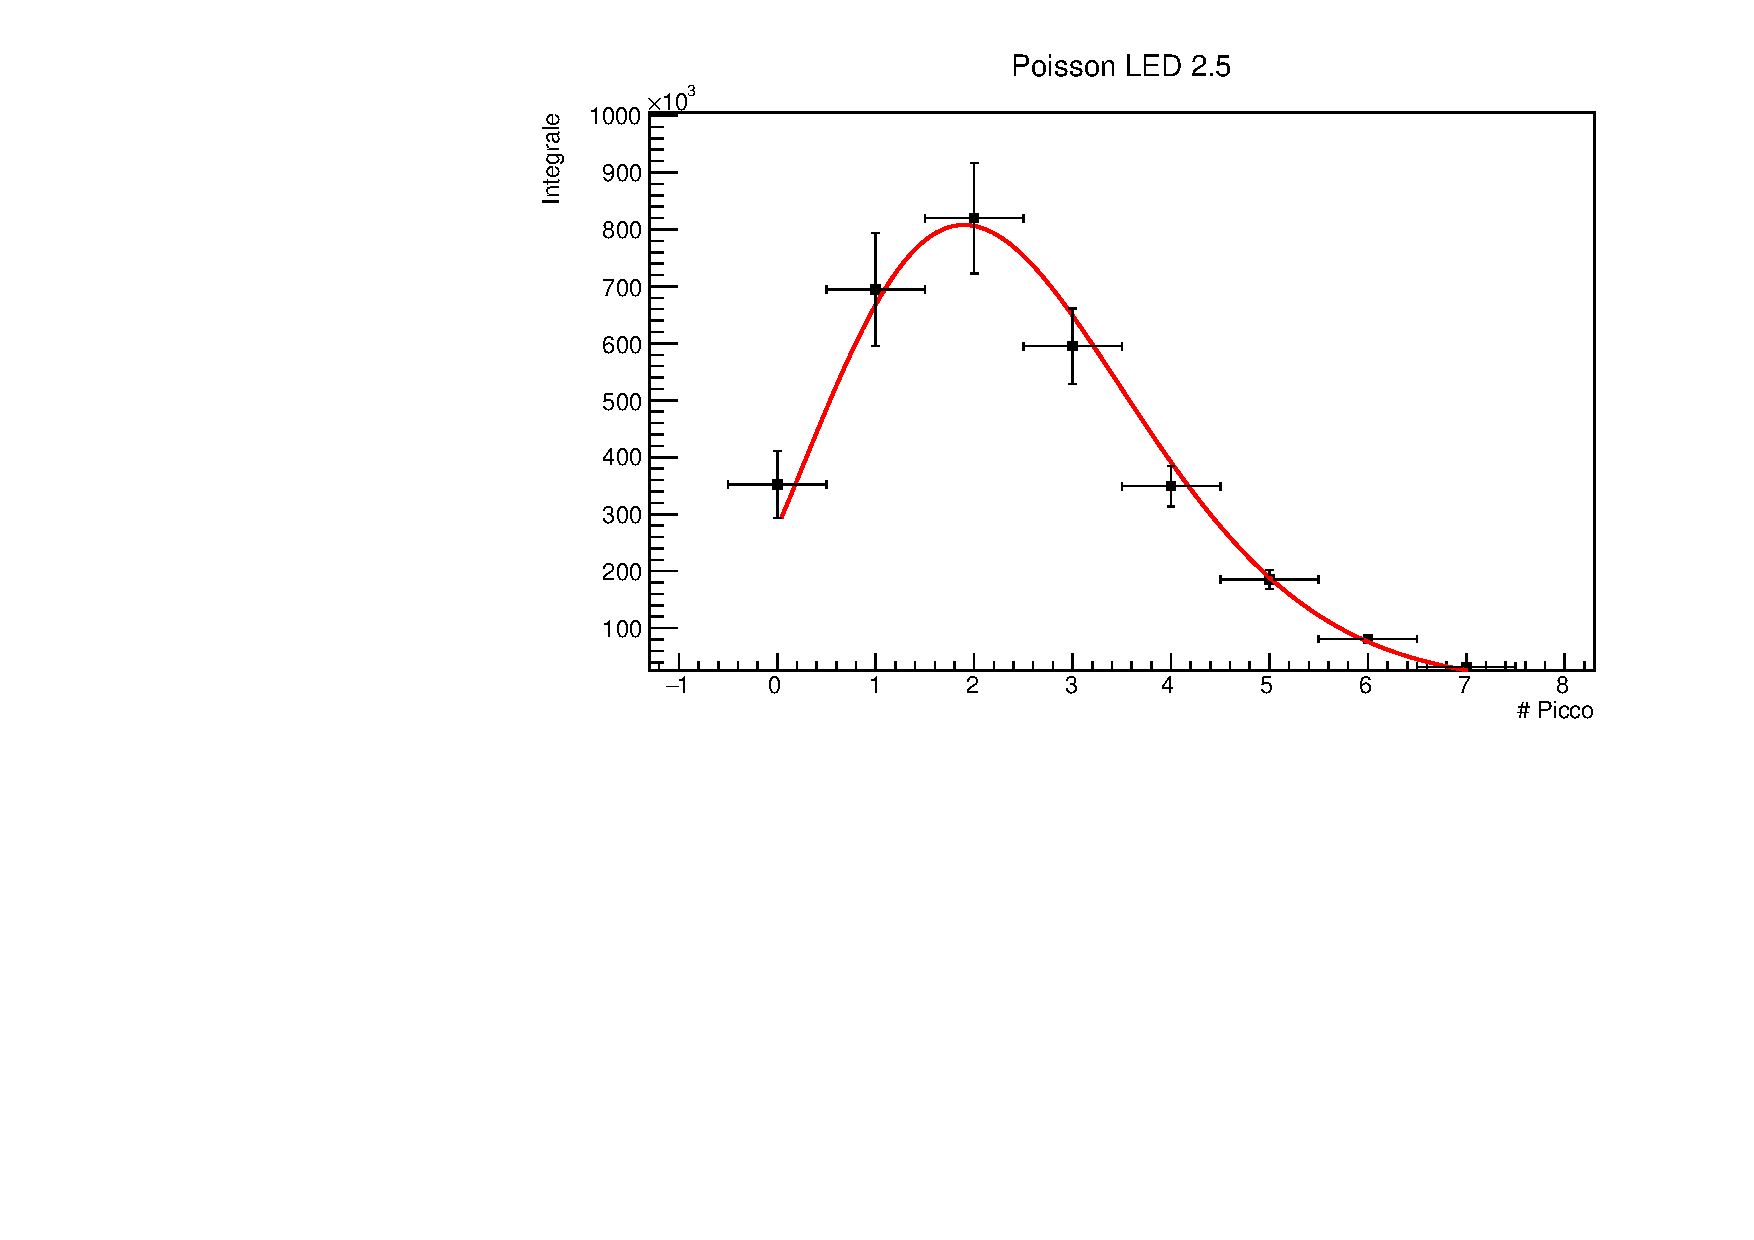
\includegraphics[width=7.7cm]{img/pois25.pdf} }}%
    \subfloat[]{{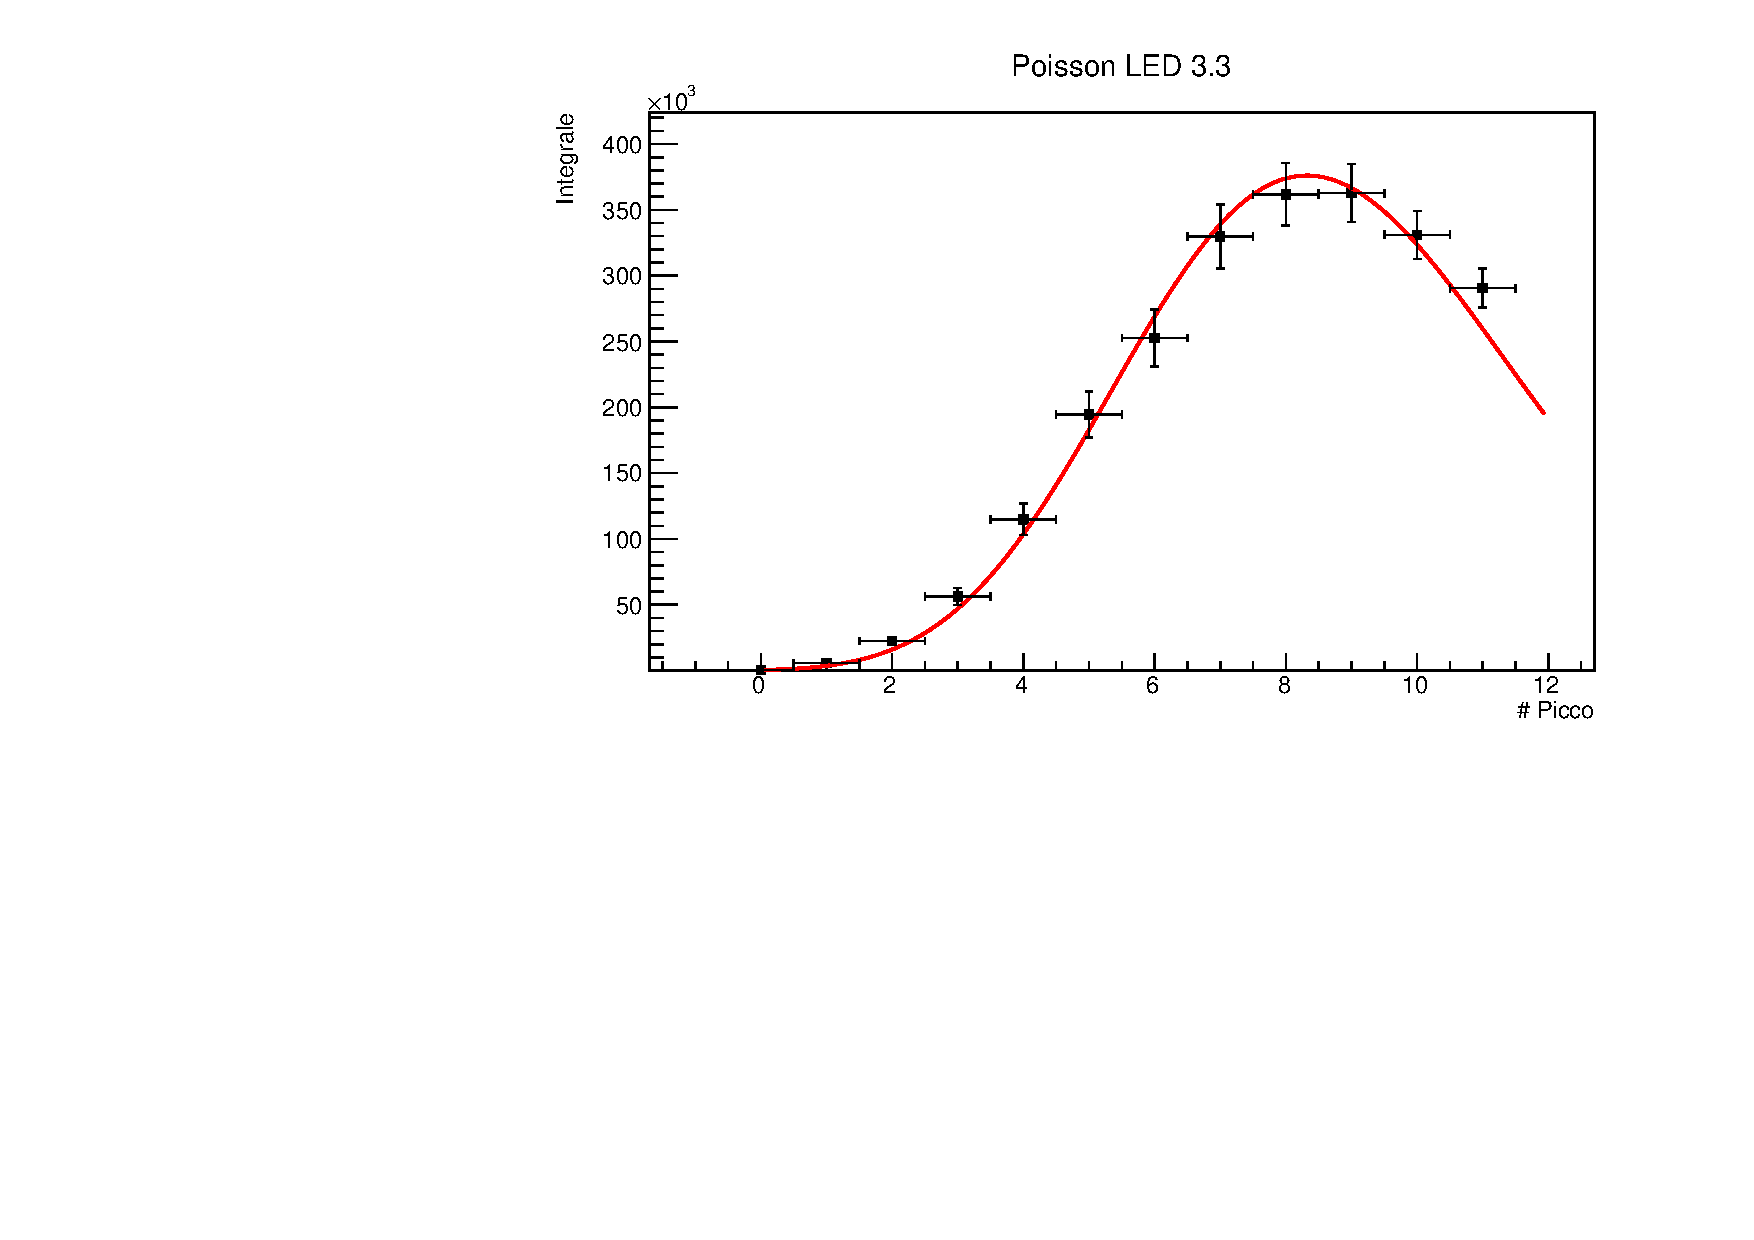
\includegraphics[width=7.7cm]{img/pois33.pdf} }}%
\caption{Fit della distribuzione di Poisson sugli integrali dei picchi.}
\end{figure}
Le distribuzioni di Poisson hanno risultati vicini alle previsioni, tenendo conto però che gli errori sui dati sono piuttosto elevati dato il metodo molto approssimato. Per il led a 2.5 il numero medio di fotoelettroni emesso è di $\mu_{2.5}=\left(2.4\pm0.2\right)$, per il led a 3.3 il numero medio di fotoelettroni è di $\mu_{3.3}=\left(8.8\pm0.2\right)$.
\begin{table}[!h]
\begin{center}
\begin{tabular}{|c|c|c|}
\hline
\multicolumn{1}{|l|}{Parametro} & \multicolumn{1}{l|}{Valore} & \multicolumn{1}{l|}{Errore}  \\ \hline\hline
$M_{2.5}$                               & $3.1\times10^{6} $                     & $0.3\times10^{6}  $                          \\ \hline
$\mu_{2.5}$                               & 2.4                       & 0.2                             \\ \hline \hline
$M_{3.3}$                               & $2.8\times10^{6} $                   & $0.1\times10^{6} $                        \\ \hline
$\mu_{3.3}$                               & 8.8                      & 0.2                             \\ \hline
\end{tabular}
\end{center}
\caption{Risultati dei fit.}
\end{table}
\\Per il LED 2.5, il fit riporta un $\chi^2$ di 0.46 con p-value 100\%, mentre per il LED 3.3 il fit riporta un $\chi^2$ di 2.27 con p-value 99\%.
Infine si è svolto un fit lineare che sottolineasse la linearità fra la $\sqrt{N}$ e la deviazione standard $\sigma$.
\begin{figure}[!h]
\centering
    \subfloat[]{{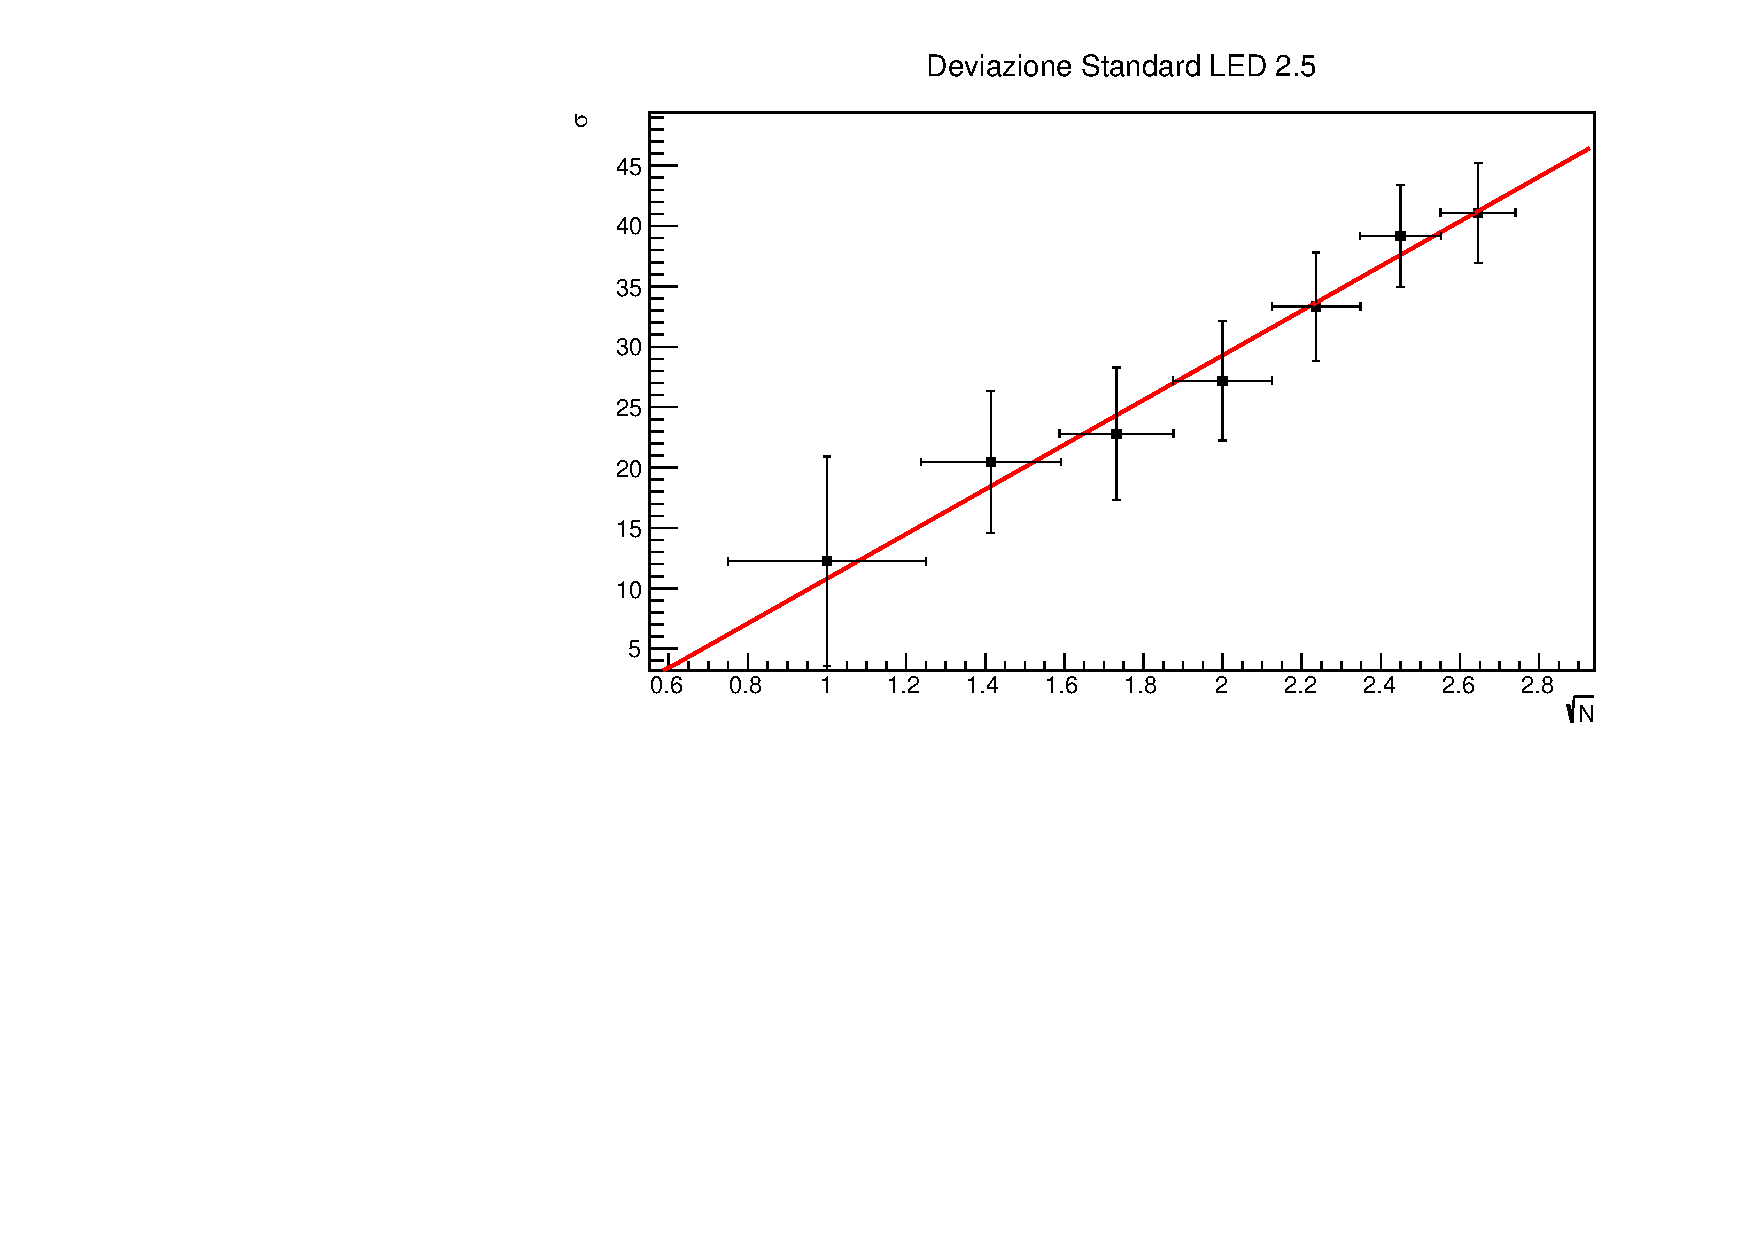
\includegraphics[width=7.7cm]{img/sigma25.pdf} }}%
    \subfloat[]{{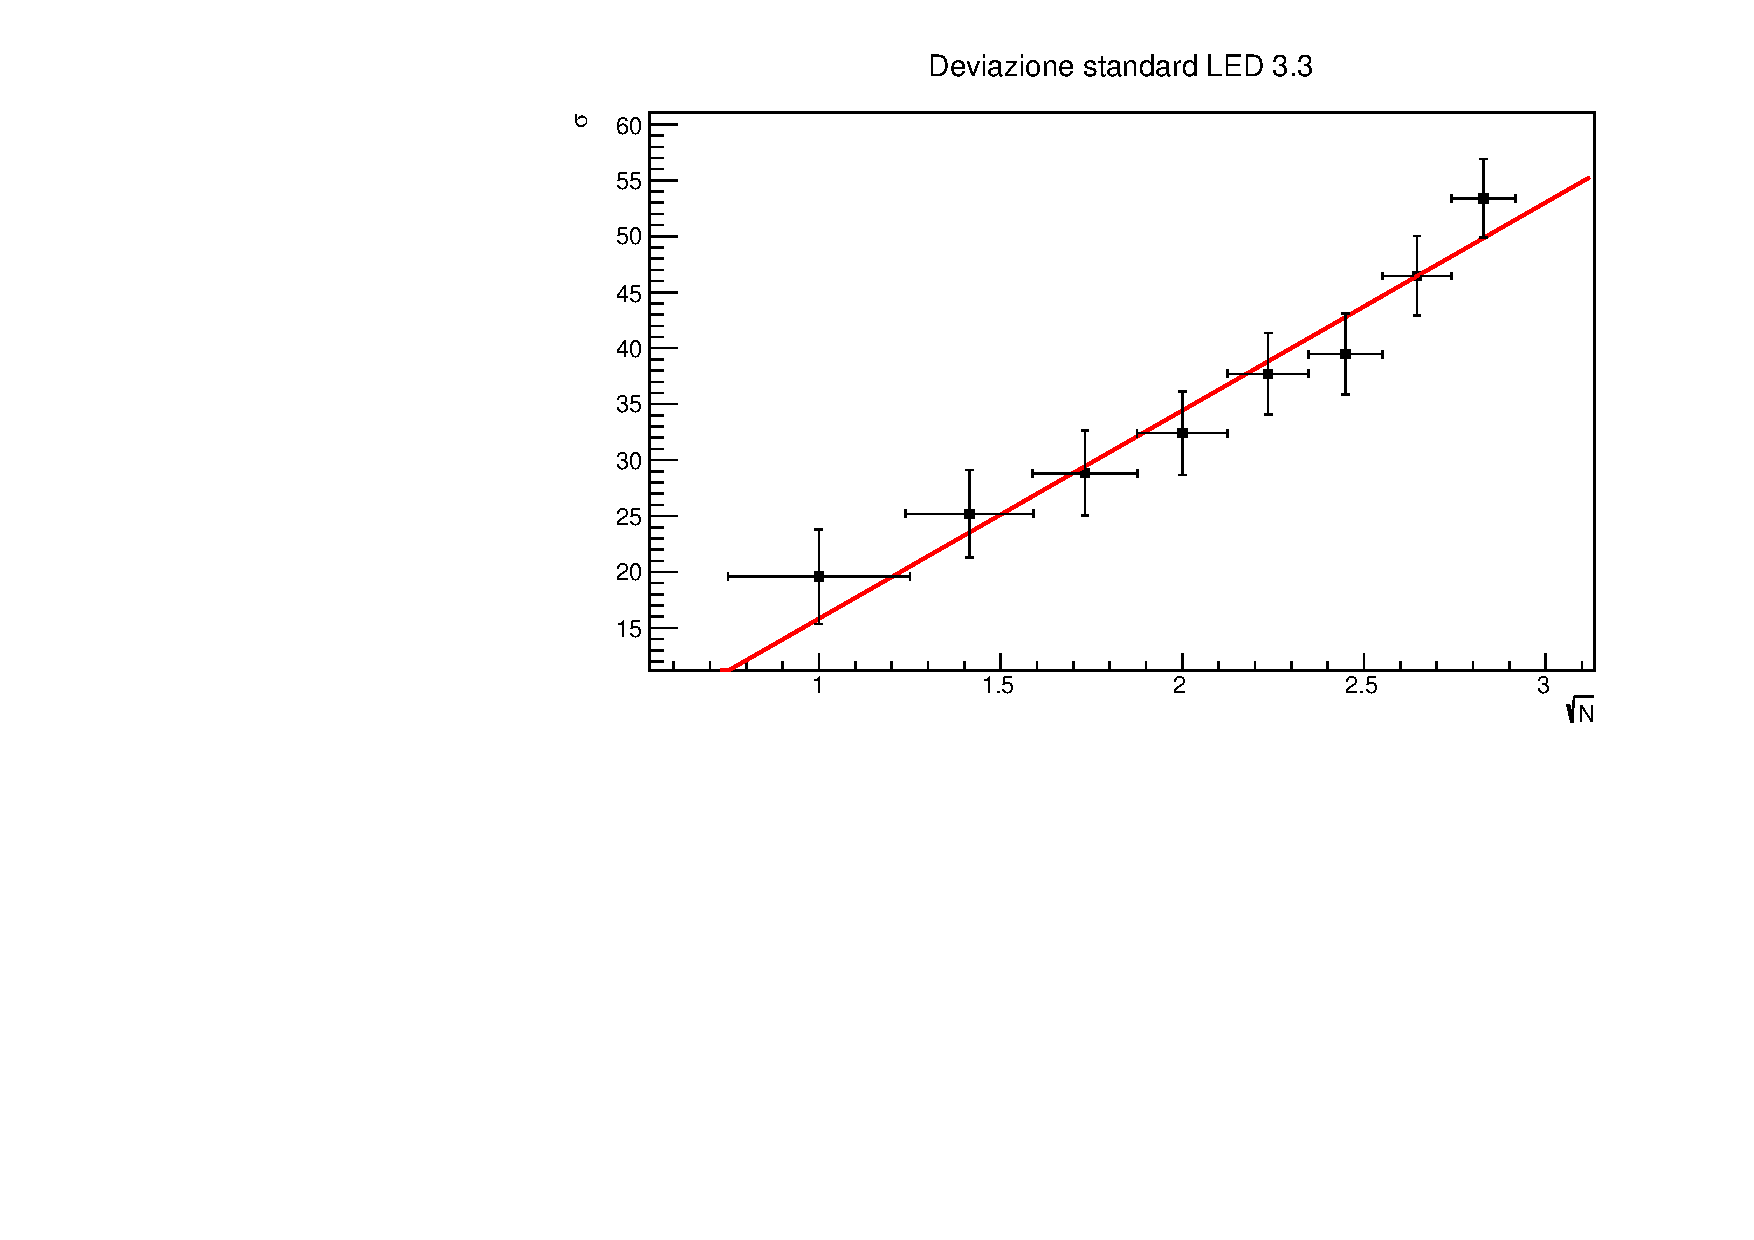
\includegraphics[width=7.7cm]{img/sigma33.pdf} }}%
\caption{Fit lineare sulle deviazioni standard dei picchi.}
\end{figure}
\begin{table}[!h]
\begin{center}
\begin{tabular}{|c|c|c|}
\hline
\multicolumn{1}{|l|}{Parametro} & \multicolumn{1}{l|}{Valore} & \multicolumn{1}{l|}{Errore}  \\ \hline\hline
$m_{2.5}$                               & 18                      &5                  \\ \hline
$q_{2.5}$                               & -8                     & 10                             \\ \hline \hline
$m_{3.3}$                               & 19                   & 3                       \\ \hline
$q_{3.3}$                               & -2                      & 7                            \\ \hline
\end{tabular}
\end{center}
\caption{Risultati dei fit.}
\end{table}
\newpage
Per il LED 2.5, il fit riporta un $\chi^2$ di 0.44 con p-value 99\%, mentre per il LED 3.3 il fit riporta un $\chi^2$ di 2.26 con p-value 89\%.
\\Come si può notare, gli errori su questi dati sono molto elevati, per cui è facile che una regressione lineare abbia esito positivo, per determinare se fossero effettivamente correlati, si è valutato il coefficiente di Pearson, risultato essere 0.9 per entrambe, indicando quindi che i dati sono linearmente proporzionali, come atteso. \\Chiaramente, anche se non particolarmente significativo viste le incertezze, l'intercetta della regressione è compatibile con l'origine in entrambi i casi.
\subsection*{Conclusioni}
L'esperienza di caratterizzazione del SiPM non ha dato i risultati attesi. Le principali difficoltà che si sono riscontrate sono state l'impostazione del setup sperimentale e la presa dati con l'eventuale valutazione in tempo reale. I dati presi, nonostante fossero state seguite le indicazioni di utilizzo, sono risultati essere molto rumorosi, facilmente risolvibile ripetendo la misura integrando su un maggior intervallo di tempo. Inoltre, conoscendo più approfonditamente l'analisi multipicco, si sarebbero potuti impostare parametri in modo da ottimizzare l'analisi a posteriori. Nonostante ciò il metodo approssimato utilizzato ha comunque dato dei risultati accettabili, non molto distanti dalle previsioni; ma comunque con degli errori molto elevati e quindi i risultati sono poco significativi.
\begin{center}
\adfopenflourishleft\quad\adfast3\quad\adfopenflourishright
\end{center}
\begin{thebibliography}{}
\bibitem{1} Covarelli R., \emph{Slides sugli esperimenti}, Campusnet, 2019.
\bibitem{2} Leo W. R., \emph{Techniques for Nuclear and Particle Physics experiments}, Springer-Verlag.
\bibitem{3} Knoll G. F., \emph{Radiation Detection and Measurement}, Wiley and Sons.
\bibitem{4} Caccia M. et al., \emph{An educational kit based on a modular Silicon Photomultiplier system}, CAEN ED3127.
\end{thebibliography}
\end{document}
